\documentclass[a4paper, 12pt]{article}

%---------------------------------------------------------------
% Layout
%---------------------------------------------------------------
\usepackage{pdfpages}
\usepackage{pdflscape}			  		% To rotate page in PDF using \begin{landscape}
\usepackage{rotating}					  % To rotate page in PDF using \begin{sidewaystable}

%---------------------------------------------------------------
% Formatting
%---------------------------------------------------------------
\usepackage{float}							% Placing inputs in current section
\usepackage{enumerate}				   % Personalizes the enumerate style
\usepackage{titlesec}

%---------------------------------------------------------------
% Math
%---------------------------------------------------------------
\usepackage{amsmath} 						% For command eqref
\usepackage{amssymb} 						% For math fonts
\usepackage{dsfont}								% More math fonts (e.g. indicator function)

%---------------------------------------------------------------
% Figures and Tables
%---------------------------------------------------------------
\usepackage{standalone}			  % To compile sub-files as part of main document
\usepackage{afterpage}				% Places float one page after it is mentioned
\usepackage[labelsep=period,labelfont=bf]{caption} % Dot separator, boldfaced

% Figures
\usepackage{graphicx} 				% Needed for \includegraphics
\usepackage[outdir=./]{epstopdf}  % Avoids errors when calling figures
\usepackage{subcaption}	    	  % Multi-panel figure: \begin{subfigure}[t]{\textwidth}

% Tables (extensions to the standard tabular environment)
\usepackage{booktabs}			  % Needed for \toprule, \midrule, \bottomrule
\usepackage{tabularx}				% Creates paragraph-like columns
\usepackage{threeparttable}		 % Includes a structured note section
\usepackage{longtable} 			   % For multi-page tables, note section needs package threeparttablex
\usepackage{multirow}			   % To add entries with multiple rows
\usepackage{bigstrut} 			 	 % Needed for \bigstrut
\usepackage{siunitx}				 % To align the decimal points

%---------------------------------------------------------------
% Hyperlinks
%---------------------------------------------------------------
\usepackage[colorlinks=true]{hyperref} 	% Creates hyperlinks, 'true' gets rid of awful boxes
\usepackage{xcolor}
\definecolor{c1}{rgb}{0,0,1} 				  % Blue
\definecolor{c2}{rgb}{0,0.3,0.9} 			% Light blue
\definecolor{c3}{rgb}{0.3,0,0.9} 			% Red blue
\hypersetup{
	linkcolor={black}, 								% Internal links
	citecolor={black}, 								% Citations
	urlcolor={black} 									 % External links/urls
}

%---------------------------------------------------------------
% Special Characters
%---------------------------------------------------------------
\usepackage[utf8]{inputenc}	% Handles accented characters (declare a character set to guarantee the same output on all systems)

%---------------------------------------------------------------
% References
%---------------------------------------------------------------
\usepackage[style=ext-authoryear,maxbibnames=99,maxcitenames=2,uniquelist=false,uniquename=false,dashed=false,doi=false,isbn=false,url=false,backend=biber]{biblatex} 
\usepackage[style=american]{csquotes}
\usepackage{xpatch}

% Citations separated by a comma
\renewcommand\multicitedelim{\addcomma\space}

% Comma or dot after author
\xpretobibmacro{date+extradate}{%
	\ifentrytype{incollection}{
		\setunit{\addcomma\space}%
	}{
		\setunit{\addperiod\space}%
	}
}{}{}

% No pp. before pages
\DeclareFieldFormat[article]{pages}{#1}
\DeclareFieldFormat[report]{pages}{#1}

% Remove dot after year
\DeclareDelimFormat[bib]{nametitledelim}{\addspace}

% Title in quotations and type not in italics
\DeclareFieldFormat[report]{title}{\mkbibquote{#1\isdot}}

% Omit fields for article
\AtEveryBibitem{%
	\ifentrytype{article}{
		\clearfield{urldate}%
		\clearfield{review}%
		\clearfield{issn}%
		\clearfield{month}%%
	}{}
}

% Comma after first author name
\AtBeginBibliography{%
	\renewcommand*{\finalnamedelim}{%
		\ifentrytype{incollection}{%
			\ifnumgreater{\value{liststop}}{2}{\finalandcomma}{}
			\addspace\bibstring{and}\space
		}{
			\finalandcomma
			\addspace\bibstring{and}\space
		}
	}%
}

% No in: before journal or report title, and custom for others
\renewbibmacro{in:}{%
	\ifboolexpr{%
		test {\ifentrytype{article}}%
		or
		test {\ifentrytype{report}}%
	}{}
	{\printtext{\bibstring{in}\space}%
		\printunit{\space}%
	}%
}

% Patch the drivers for incollection
\DefineBibliographyStrings{english}{byeditor = {edited by}}

% Add bibliography database
\addbibresource{../References/library2.bib}

%---------------------------------------------------------------
% Appendix
%---------------------------------------------------------------
\usepackage{appendix}

%---------------------------------------------------------------
% Page Settings
%---------------------------------------------------------------
\usepackage[margin=1in]{geometry} 					% Sets the margins of the file
\usepackage{fancyhdr} 						% Needed for head and foot options
\usepackage{setspace}
\doublespacing
\AtBeginDocument{								 % Avoids excesive spacing b/w floating objects
	\addtolength\abovedisplayskip{-0.2\baselineskip}
	\addtolength\belowdisplayskip{-0.2\baselineskip}
}
\newcommand{\sectitlespace}{\vspace{0.1in}}
\sloppy 								 			% Try to avoid hyphens
\makeatletter
\def\@fnsymbol#1{\ensuremath{\ifcase#1\or \dagger\or *\or
		\mathsection\or \mathparagraph\or \|\or **\or \dagger\dagger
		\or \ddagger\ddagger \else\@ctrerr\fi}}
\makeatother

%---------------------------------------------------------------
% Subcaptions
%---------------------------------------------------------------
% Notes after figures following Jörg Weber
\newcommand{\figtext}[1]{
	\vspace{-1ex}
	\captionsetup{justification=justified,font=footnotesize}
	\caption*{#1}
}

\newcommand{\fignote}[1]{\figtext{\emph{Note:~}~#1}}
\newcommand{\fignotes}[1]{\figtext{\emph{Notes:~}~#1}}

% Notes after tables
\newcommand{\tabnote}[1]{
	\begin{tablenotes}[para,flushleft]
		\footnotesize \emph{Notes:~}~#1
	\end{tablenotes}
}

%---------------------------------------------------------------
% Tables
%---------------------------------------------------------------
\newcolumntype{C}{>{\centering\arraybackslash}X}

%---------------------------------------------------------------
% Variable Definitions
%---------------------------------------------------------------
\providecommand{\tiie}{TIIE28D}
\providecommand{\lastobs}{June 2023}
\providecommand{\lastobsfx}{November 2021}
\providecommand{\lastobsflwbdm}{June 2023}
\providecommand{\lastobsflwtic}{January 2023}
\providecommand{\breakdatefx}{October 31, 2014}
\providecommand{\breakdateyc}{April 30, 2015}
\providecommand{\breakdatecetes}{December 15, 2016}
\providecommand{\breakdatebonos}{February 11, 2021}
\providecommand{\idxt}{t}
\providecommand{\idxh}{h}
\providecommand{\idxsfwd}{\idxt+\idxh}
\providecommand{\idxslag}{\idxt-1}
\providecommand{\yld}{y}
\providecommand{\ctrls}{z}
\providecommand{\hld}{H}
\providecommand{\depvar}{\Delta \yld_{\idxt}}
\providecommand{\paramB}{\beta}
\providecommand{\intrcpt}{\paramB_{0}}
\providecommand{\slopetrgt}{\paramB_{1}}
\providecommand{\slopepath}{\paramB_{2}}
\providecommand{\assets}{X}
\providecommand{\factors}{F}
\providecommand{\loadings}{\Lambda}
\providecommand{\rotated}{Z}
\providecommand{\rmatrix}{U}
\providecommand{\rtdone}{\rotated_{1}}
\providecommand{\rtdtwo}{\rotated_{2}}
\providecommand{\rtdonereg}{Target_{\idxt}}
\providecommand{\rtdtworeg}{Path_{\idxt}}
\providecommand{\dimobs}{T}
\providecommand{\dimassets}{n}
\providecommand{\dimfactors}{k}
\providecommand{\dimnull}{\dimfactors_{0}}
\providecommand{\dimsassets}{\dimobs \times \dimassets}
\providecommand{\dimsfactors}{\dimobs \times \dimfactors}
\providecommand{\dimsloadings}{\dimfactors \times \dimassets}
\providecommand{\errorreg}{\varepsilon_{\idxt}}
\providecommand{\errorfac}{\zeta}

%---------------------------------------------------------------
% Equations
%---------------------------------------------------------------
\newcommand{\eqPCA}{\assets = \factors \loadings + \errorfac}
\newcommand{\eqRotation}{\rotated = \factors \, \rmatrix}
\newcommand{\eqTwoFacP}{\depvar = \intrcpt + \slopetrgt \rtdonereg + \slopepath \rtdtworeg + \errorreg}
\newcommand{\eqLPrhs}{\beta^{1}_{\idxh} \; \rtdonereg +  \beta^{2}_{\idxh} \; \rtdtworeg + \eta^{'}_{\idxh} \ctrls_{\idxslag}  + u_{\idxsfwd}}
\newcommand{\eqLPprices}{\yld_{\idxsfwd} = \alpha^{1}_{\idxh} + \alpha^{2}_{\idxh} \; \yld_{\idxslag} + \eqLPrhs} 
\newcommand{\eqLPflows}{\hld_{\idxsfwd} = \alpha^{1}_{\idxh} + \alpha^{2}_{\idxh} \; \hld_{\idxslag} + \eqLPrhs} 

\begin{document}
%---------------------------------------------------------------
% Title Page
%---------------------------------------------------------------
\title{Do Central Bank Words Matter in Emerging Markets? Evidence from Mexico\thanks{\protect\linespread{1}\protect\selectfont I am particularly grateful to Jonathan Wright for insightful discussions and feedback, the editor Enzo Dia and three anonymous reviewers for their insightful comments and suggestions. I also thank Derin Aksit, Laurence Ball, Enrique Batiz, Christopher Carroll, Lalit Contractor, Juan Pablo de la Mora, Jorge Luis García Ramírez, Karlye Dilts Stedman, Gregory Duffee, Eric Fischer, Raúl Ibarra Ramírez, Olivier Jeanne, Fabrizio López Gallo Dey, Claudia Ramírez Bulos, Alessandro Rebucci, Ariadna Valle Carmona, and seminar participants at the 2020 Southern Finance Association meeting and Banco de México for their helpful comments and suggestions. The views in this paper are the sole responsibility of the author and should not be interpreted as reflecting the views of Banco de México or any other person associated with it. All remaining errors are mine.}
}
\author{Pavel Solís\thanks{\protect\linespread{1}\protect\selectfont Senior Economist, Financial Stability Division, Banco de México, Av. 5 de Mayo No. 1, Centro, Cuauhtémoc, CDMX 06000, México. E-mail address: \href{mailto:pavel.solis@banxico.org.mx}{\texttt{pavel.solis@banxico.org.mx}}. Declarations of interest: none.}
}
\date{2023}

\maketitle	\vspace{-4ex}

%---------------------------------------------------------------
% Abstract
%---------------------------------------------------------------
\begin{abstract}
	This paper analyzes the price and quantity effects of monetary policy statements in an emerging market economy. Surprises in monetary policy are identified using intraday data on asset prices around monetary policy announcements in Mexico. I find that asset prices and the portfolio flows of domestic and foreign investors respond strongly and persistently to both news about the policy rate and guidance about its future path communicated via statements. The ability to manage expectations about future policy via statements is thus not exclusive to central banks in advanced economies and does not require the zero lower bound to be binding. 
	
	\vspace{.5cm}
	\noindent \textit{Keywords}: Monetary policy surprises, exchange rate, yield curve, portfolio flows, emerging markets, high-frequency data.
	
	\noindent \textit{JEL Classification}: E52, E58, E43, F31, G14. 
	\vfill
	
	\pagebreak
\end{abstract}

%---------------------------------------------------------------
% Contents
%---------------------------------------------------------------
\section{Introduction}
Monetary policy in emerging markets is generally viewed in terms of interest rate policies. For advanced economies, however, it is also associated with forward guidance and asset purchases. Are central banks in emerging markets limited to interest rate policies? On the one hand, committing to a future policy seems unnecessary when the policy rate is unconstrained by the zero lower bound, as is generally the case for emerging markets. On the other hand, an inflation targeting regime and well-anchored inflation expectations allow them to pursue more forward-looking policies so as to reduce policy uncertainty. 

This paper studies whether the monetary policy in an emerging market economy is conducted exclusively through adjustments in the level of the policy rate or, also, by communicating information about its future policy via statements. 
To address this question, I first construct a new dataset of intraday changes in swap rates around regular monetary policy announcements in Mexico from 2011 to 2023,\footnote{The swaps reference an interbank interest rate that closely follows the policy rate.} and use it to identify monetary policy surprises following the methodology proposed by \textcite{GSS:2005a};\footnote{Their methodology identifies surprises directly from asset prices, it does not involve textual analysis.} 
I then assess the price \textit{and} quantity effects of those surprises by analyzing the response of the exchange rate, bond yields and the portfolio flows of domestic and foreign investors.

Mexico offers an ideal setting to study this question. It is a small open economy with a credible inflation targeting regime \parencite{DePooter_etal:2014,Beauregard_etal:2021}, a market-based exchange rate \parencite{IlzetzkiReinhartRogoff:2019}, and relatively liquid financial markets\footnote{In particular, the sovereign local currency bond market has a diversified (domestic and foreign) investor base, a highly liquid repo market, effective systems for market making, settlement and clearing, and bonds included in global benchmark indices \parencite{OECDsbo:2016}. Although foreign investors are an important driver of the liquidity premium in Mexican fixed-rate bonds \parencite{CFS:2021}, the market is not dependent on them, as is the case for other emerging markets \parencite[see Table A B.20 in][]{OECDsbo:2023}.}. 
Several emerging markets share similar characteristics \parencite{Ruch:2021,IlzetzkiReinhartRogoff:2019,OECDsbo:2020}, so the analysis in this paper can serve as a benchmark for understanding the effects of their monetary policy statements. In addition, the Mexican central bank collects a unique dataset of daily holdings of Mexican government securities that allows me to better understand the transmission mechanisms of its monetary policy.\footnote{Cross-border capital flows (including portfolio flows, foreign direct investment, and banking flows) are reported quarterly, although some sources report portfolio flows monthly and at most weekly.} 

I find that Banxico, the Mexican central bank, conducts its monetary policy by communicating two types of information via statements: news about the policy rate and guidance about its future path. 
They are henceforth referred to as target and path surprises, respectively.\footnote{Path surprises by emerging market central banks could also be considered as communication surprises or as a subtle form of forward guidance. \textcite{Kuttner:2018} notes that although there is no consensus in the literature of what constitutes forward guidance, the likely trajectory of the policy rate communicated near the zero lower bound is more explicit than under a conventional regime.} 
I show in particular that path surprises are closely related to information in statements about the future path of the policy rate, consistent with the evidence for advanced economies when the zero lower bound was not binding \parencite[e.g.,][]{GSS:2005a}. 
The fact that path surprises are not only available but actually used by Banxico suggests that central banks in emerging markets do have the ability to manage expectations about future policy via statements, as long as the path surprises are credible. 

Banxico's target and path surprises influence asset prices and portfolio flows. 
The analysis relies on a high-frequency event study and local projections to quantify the contemporaneous and persistent effects  of target and path surprises on asset prices and portfolio flows. High-frequency event studies overcome endogeneity concerns by isolating the surprise component of monetary policy decisions \parencite{NakamuraSteinsson:2018JEP}, while local projections are more robust to model misspecification than vector autoregressions \parencite{Jorda:2005}. The structural test developed by \textcite{BaiPerron:2003} complements the analysis to assess whether the sensitivity to monetary policy has changed over time. 

Target and path tightening surprises appreciate the local currency, in line with standard open economy models. A 25 basis point target or path tightening surprise appreciates the currency by about 0.6\% and 0.3\%, respectively, over the sample. However, the role of both surprises shifted at the end of 2014, a period of declining oil prices and uncertainty about the end of the zero lower bound era in the U.S. The exchange rate response is stronger and persistent to path surprises before the end of 2014, and to target surprises afterwards. A 25 basis point target (post-2014) or path (pre-2014) tightening surprise would appreciate the currency by 1.3\%. 
Both surprises occurred more frequently post-2014, which suggests that investors in the forex market may give more weight to information about the \textit{future} stance of monetary policy in periods of relative stability, but more weight to the \textit{current} monetary policy stance when they are frequently surprised by the central bank. In any case, both type of surprises play an important role in the transmission of monetary policy to the exchange rate, a vital channel for open economies.

Target and path tightening surprises also flatten the yield curve. 
Medium- and long-term yields tend to react more to path than to target surprises on-impact, consistent with the evidence for the U.S. when its policy rate was not constrained by the zero lower bound \parencite{GSS:2005a,Swanson:2021}. 
Both surprises have persistent effects on the yield curve days after an announcement, but their role shifted in early 2015, still in the context of declining oil prices and uncertainty about the normalization of the monetary policy in the U.S. 
Bond yields' response is stronger to target surprises ahead of early 2015, and to path surprises afterwards. The timing of the change for the exchange rate and bond yields is close enough to suggest that forex investors weight target and path surprises differently to bond investors. 
Regardless, path surprises improve the implementation of monetary policy in Mexico by affecting medium- and long-term yields to the extent they influence the spending decisions of households and firms. 

Domestic and foreign investors rebalance their debt portfolios in response to target and path surprises. This rebalancing effect occurs between domestic and foreign investors as well as across different types of domestic investors. For instance, the evidence suggests that after a tightening of the monetary stance through target and path surprises, some domestic investors (firms and households) position themselves in the short end of the yield curve, while foreign investors prefer exposure to the long end.
Foreign investors thus participate in the transmission of the local monetary policy.\footnote{In case foreigners retreat from the market, domestic investors step in (see section \ref{sec:flowsdaily}).} 
Finally, investors take time to rebalance their portfolios. This sluggish response by investors supports the evidence of a persistent response by the exchange rate and bond yields just mentioned, and is consistent with the literature on slow-moving capital in asset pricing \parencite{Duffie:2010}. 

Banxico therefore does not conduct monetary policy exclusively using target surprises. Path surprises have an equally important role in the transmission of monetary policy. Moreover, the relative influence of each policy can change over time depending on macroeconomic conditions and institutional arrangements. This evidence shows that at least one emerging market central bank is clearly not limited to interest rate policies. 
The multidimensionality of monetary policy \parencite{GSS:2005a,Altavillaetal:2019,Swanson:2021} is thus not exclusive to central banks in advanced economies and does not require the zero lower bound to be binding.

This paper contributes to the literature in three respects. 
First, it assesses the role of high-frequency identified path surprises in an emerging market economy. 
The literature on the multidimensionality of monetary policy has hitherto concentrated on advanced economies,\footnote{ \textcite{Blinderetal:2008} review the literature on the influence of central bank communications on financial markets but mainly for advanced economies. Some evidence exists for emerging markets using content analysis to classify communications \parencite{SuAhmadWood:2019}, yet the approach is prone to subjectivity.} and intraday data is rarely used for emerging markets. 
Second, the effects of target and path surprises are not only analyzed on asset prices but on daily portfolio flows to better understand the transmission mechanisms of monetary policy. The literature for advanced economies generally considers only the effects on prices (not quantities), while for emerging markets, it mostly focuses on target (not path) surprises \parencite{Kohlscheen:2014,Solis:FX}. 
Third, this paper takes the perspective of the host country when analyzing the effects of its monetary policy on incoming portfolio flows. Traditionally, the literature on monetary policy spillovers takes the perspective of the home country.\footnote{This literature documents significant flows into financial assets in emerging markets after the global financial crisis \parencite{FratzscherLoDucaStraub:2018}. \textcite{HausmanWongswan:2011} show that stock prices respond more to U.S. target surprises, that exchange rates and long-term yields respond more to U.S. path surprises, and that short-term yields respond to both. \textcite{BowmanLondonoSapriza:2015} and \textcite{Fischer:2020} show that U.S. monetary policy surprises are particularly relevant for the local currency sovereign yields.} 
As far as I know, this is the first paper to show evidence on the portfolio rebalancing effect of monetary policy using daily flow data and on how foreign investors respond to the monetary policy of an emerging market.

The rest of the paper is structured as follows. 
Section \ref{sec:mpsidentification} describes how monetary policy surprises are identified. 
Section \ref{sec:statements} shows that Banxico uses two types of monetary policy surprises. Sections \ref{sec:assets} and \ref{sec:flows} respectively characterize the response of asset prices and portfolio flows to both types of surprises. The last section concludes.


\section{Identification of Monetary Policy Surprises} \label{sec:mpsidentification}
This section summarizes the relevant institutional details for the identification of the monetary policy surprises. It also describes the asset prices used in the analysis. 

The Bank of Mexico, also known as Banxico, is an independent central bank that follows an inflation targeting regime since 2001. 
Its inflation target is 3\% with a range of \(\pm\) 1\%, and its monetary policy instrument is the overnight interbank interest rate. 
A Governing Board comprising a governor and four deputy governors meets on average eight times a year to discuss monetary policy; the announcements of its decisions are made via statements released at 1 p.m. local time on dates (usually Thursdays) that are published ahead of time.\footnote{Previously, Banxico conducted monetary policy by setting a quantitative target for reserves and by expressing monetary conditions in basis points (before 2008), the Governing Board met more frequently (before 2011), and the announcements were made at 9 a.m. local time (before 2015), see \textcite{Solis:FX}.} 
\textcite{Solis:FX} provides the dates and times of the announcements.

This paper uses swap rates to measure surprises in monetary policy decisions. 
The swaps market in Mexico references the 28-day interbank interest rate (\tiie), an interbank interest rate denominated in local currency that serves as a benchmark for banking loans in the country and that closely follows the policy rate.\footnote{The average spread between the \tiie{} and the policy rate is around 30 basis points. Since the spread exhibits small variation, it essentially cancels out when computing changes in swap rates.} 
Banxico reports the \tiie{} once a day based on quotes submitted by commercial banks. 
The 3-month swap of the \tiie{} is the main local derivative. 
\textcite{Solis:FX} uses it to capture surprises in the policy rate. 
This paper extends his analysis by considering a broader sense of monetary policy surprises given that the adoption of inflation targeting and well-anchored inflation expectations arguably allowed Banxico to pursue more forward-looking policies. 

I consider swaps with maturities up to one year. 
Like other central banks, Banxico communicates information about its monetary policy outlook via statements. 
This information might influence market expectations about future policy actions. 
Unlike in several countries after the global financial crisis and the Covid-19 pandemic, the policy rate in Mexico has 
not been constrained by the zero lower bound. As a consequence, Banxico's monetary policy statements include information about future policy actions within a year out at most, it does not need to commit to a predetermined policy path for longer periods. 
Moreover, using maturities up to one year is consistent with the approach of \textcite{GSS:2005a} for the U.S. before the global financial crisis.\footnote{ \textcite{Swanson:2021} argues for including maturities of more than one year out if the policy rate is constrained by the zero lower bound and the central bank uses unconventional monetary policy tools.} 

Asset price changes are calculated on intraday windows containing regular monetary policy announcements. 
The monetary policy surprises use intraday differences from 10 minutes before to 20 minutes after each announcement for swaps with maturities of 3, 6, 9 and 12 months.\footnote{When no information is available at any of those times, the next available quote is used instead. If they are still not available using wider windows for the day, the open and close quotes are used instead. Those cases are rare, they only happen on a few days for some swaps.} 
To measure the effects of the surprises, intraday differences over the same windows are also calculated for assets that are closely related to monetary policy; namely, the Mexican peso (MXN) per U.S. dollar (USD) exchange rate and the yields of fixed-rate bonds issued by the Mexican government with maturities of  2, 5, 10 and 30 years.\footnote{ The Mexican government issued 10- 20- and 30-year fixed-rate local-currency bonds for the first time in 2001, 2003 and 2006, respectively, following the implementation of a debt management strategy to develop its debt market that started in 2000 \parencite{JeanneauTovar:2008,Banxico:2014}.} 
For yields, the change is calculated directly using quotes before and after the announcements; for the exchange rate, 100 times log differences are used to approximate the percentage change (or return) over the window.\footnote{ All the results discussed below using tight 30-minute windows remain using wider 50-minute windows, starting 20 minutes before and ending 30 minutes after each monetary policy announcement.} 

All the asset price information comes from Bloomberg. 
The data to calculate the intraday differences for the swap rates and the exchange rate are available since 2011, and since 2013 for bond yields other than the 5-year yield for which the sample starts in December 2014. The dataset covers up to the \lastobs{} announcement. 
Between January 2011 and \lastobs, there were 99 regularly-scheduled monetary policy announcements.\footnote{Banxico held three unscheduled monetary policy meetings during that period, one in 2016 and two in 2020 due to the Covid-19 pandemic. They are excluded from the sample because the decisions in all three cases were accompanied by additional non-monetary measures \parencite[see][Appendix B]{Solis:FX}. \label{fn:extrameets}} 
Table \ref{tab:summapc} summarizes the asset price intraday changes used to obtain the surprises and to analyze their effects. The process to estimate the surprises is discussed in the next section.

\begin{normalsize}
	\begin{table}[t]
		\begin{center}
			\caption{Summary Statistics of Intraday Asset Price Changes} \label{tab:summapc}
			\begin{threeparttable}
				\begin{tabularx}{0.95\linewidth}{l*{5}C}
					\toprule
					                    &        Mean&   Std. Dev.&        Min.&        Max.&         Obs.\\
					\midrule
					\(\Delta\) 3-Month Swap&        0.07&         7.5&       -45.8&        19.5&          99\\
					\(\Delta\) 6-Month Swap&        0.18&         8.8&       -46.0&        25.5&          99\\
					\(\Delta\) 9-Month Swap&        0.09&         9.3&       -49.0&        26.5&          99\\
					\(\Delta\) 12-Month Swap&        0.31&         9.4&       -44.0&        36.5&          99\\
					FX Returns          &       -9.17&        34.4&      -165.4&        55.3&          99\\
					\(\Delta\) 2-Year Yield&       -0.19&         6.8&       -37.7&        23.9&          83\\
					\(\Delta\) 5-Year Yield&        0.13&         4.6&       -15.4&        19.1&          64\\
					\(\Delta\) 10-Year Yield&       -0.50&         4.9&       -25.8&        11.9&          83\\
					\(\Delta\) 30-Year Yield&       -0.72&         4.1&       -19.8&         8.2&          83\\
					Target Surprises    &       -0.00&         7.4&       -44.8&        18.2&          99\\
					Path Surprises      &       -0.00&         3.9&       -14.9&        11.8&          99\\
					\bottomrule
					\addlinespace[.75ex]
				\end{tabularx}
				\tabnote{This table reports summary statistics of intraday changes in swap rates and bond yields, as well as exchange rate (FX) returns around monetary policy announcements. The changes are calculated from 10 minutes before to 20 minutes after an announcement. All values are expressed in basis points. The sample includes all regular monetary policy announcements from January 2011 to \lastobs; for bond yields the sample starts on January 2013, except for the 5-year yield for which the sample period covers from December 2014 to December 2022.}
			\end{threeparttable}
		\end{center}
	\end{table}
\end{normalsize}


\section{Monetary Policy Dimensions} \label{sec:statements}
This section shows that two factors in monetary policy announcements move asset prices in Mexico. The first factor is associated with surprises about the current policy rate and the other factor, with surprises about its future path communicated via policy statements. Subsequent sections analyze how asset prices and portfolio flows respond to these factors.

\subsection{Assessing the Number of Factors}
As in \textcite{GSS:2005a}, the number of factors influencing asset prices is assessed using the matrix rank test developed by \textcite{CraggDonald:1997}. 
Let \(\assets\) be a \(\dimsassets\) matrix of asset price changes around monetary policy announcements with \(\dimobs\) observations and \(\dimassets\) asset prices, and with a factor structure given by:
\begin{equation} \label{eq:nPCA}
	\eqPCA ,
\end{equation}
\noindent in which \(\factors\) is a \(\dimsfactors\) matrix with \(\dimfactors\) unobserved factors, \(\loadings\) is a \(\dimsloadings\) matrix of factor loadings and \(\errorfac\) is white noise.
For a given number of variables \(n\), the Cragg--Donald test assesses the null hypothesis that \(\dimnull\) factors (\(\dimnull < \dimassets\)) explain most of the variability observed in the data. The test minimizes the distance between the covariance matrix of the observed data and that obtained from all the possible models with \(k_{0}\) factors. The test is a Wald statistic with an asymptotic \(\chi^2\) distribution and \( \left( \dimassets - \dimnull \right) \left( \dimassets - \dimnull + 1 \right) /2 - \dimassets \) degrees of freedom. 

The test is performed for the exchange rate and bond yields (\( \dimassets = 5 \)) to assess the number of factors they react to, and for swaps with maturities up to one year (\( \dimassets = 4 \)) to give a structural interpretation to the estimated factors. 
Inference based on the Cragg--Donald test requires to satisfy the condition \( \left( \dimassets - \dimnull \right) \left( \dimassets - \dimnull + 1 \right) /2 > \dimassets \),\footnote{ See \textcite{CraggDonald:1997} and the appendix in \textcite{GSS:2005a} for further details.} therefore \( \dimnull \) can be at most 2 for the exchange rate and the yields, and 1 for the swaps. 
To check robustness to the frequency of the data and to the sample period, the test is also performed using daily changes in asset prices around the announcements. 
Daily changes for all assets are calculated since 2004, except for the 30-year yield with data since October 2006.

Table \ref{tab:ranktests} shows that two factors characterize the responses of asset prices to monetary policy in Mexico. The null hypothesis of no factors (\(\dimnull = 0\)) is strongly rejected in all cases, so asset prices in Mexico respond at least to one factor; \textcite{Solis:FX} indeed shows that they respond to unanticipated changes in the current policy rate. The most interesting null hypotheses therefore involve one and two factors. 
The null hypothesis of one factor (\(\dimnull = 1\)) is rejected for the exchange rate and bond yields, as well as for the swaps, regardless of the data frequency and the sample period, so asset prices respond at least to two factors. A third factor is not supported by the data since the null of two factors (\(\dimnull = 2\)) cannot be rejected, even at the 10\% significance level. 
Therefore, two factors drive the response of asset prices to monetary policy announcements, which implies that the multidimensionality of monetary policy \parencite{GSS:2005a, Altavillaetal:2019,Swanson:2021} is not exclusive to advanced economies. 

\afterpage{
	\begin{normalsize}
		\begin{landscape}
			\begin{table}
				\centering
				\begin{threeparttable}
					\caption{Tests of the Number of Factors in Monetary Policy Surprises}
					\label{tab:ranktests}
					\begin{tabular}{lcccccc}
						\toprule
						& Frequency & \(H_{0}: k = k_{0}\) & Wald Statistic & Degrees of Freedom & \(p\)-value & Observations \\
						\midrule
						&  & 0 & 26.25 & 10 & 0.003 & 64 \\
						& Intraday & 1 & 11.94 & 5 & 0.036 & 64 \\
						Exchange Rate &  & 2 &  1.23 & 1 & 0.267 & 64 \\
						\cmidrule(lr){2-7}
						\& Yield Curve &  & 0 & 47.84 & 10 & 0.000 & 145 \\
						& Daily & 1 & 22.60 & 5 & 0.000 & 145 \\
						&  & 2 &  0.05 & 1 & 0.828 & 145 \\
						\cmidrule(lr){1-7}
						\multirow{4}[5]{*}{Swaps} & \multirow{2}{*}{Intraday} & 0 & 30.43 & 6 & 0.000 & 99 \\
						&  & 1 &  6.57 & 2 & 0.037 & 99 \\
						\cmidrule(lr){2-7}
						& \multirow{2}{*}{Daily} & 0 & 37.29 & 6 & 0.000 & 202 \\
						&  & 1 &  9.93 & 2 & 0.007 & 202 \\
						\bottomrule
					\end{tabular}
					\begin{tablenotes}[para,flushleft]
						\footnotesize \textit{Notes:} This table reports the results from the Cragg--Donald test. \(H_{0}\) is the null hypothesis of \(k = k_{0}\) factors against the alternative of \(k > k_{0}\) factors, where \(k_{0} = 0, 1, 2\). The sample includes all regular monetary policy announcements up to \lastobs, the starting date varies based on data availability: for the exchange rate and the yield curve, it is December 2014 (due to the 5-year yield) with intraday data and October 2006 (due to the 30-year yield) with daily data; for swaps, it is January 2011 with intraday data and January 2004 with daily data. The yield curve includes 2-, 5-, 10- and 30-year bonds. Swaps have maturities of 3, 6, 9 and 12 months.
					\end{tablenotes}
				\end{threeparttable}
			\end{table}
		\end{landscape}
	\end{normalsize}
}

Notice that two monetary policy factors in Mexico is not a recent phenomenon. 
The test using daily data since 2004 shows that asset prices have responded to two factors even before Banxico adopted its current policy rate in 2008.\footnote{The daily sample can start in 2004 because the swaps reference the \tiie{}, not the policy rate. \label{fn:sampledy}} 

In sum, asset prices react to information other than news about the policy rate on announcement days. 
I now explain how to estimate and interpret the two factors.


\subsection{Estimating the Factors} \label{sec:factors}
The factors \(\factors\), as well as their loadings \(\loadings\), in equation (\ref{eq:nPCA}) are estimated by applying principal components to the matrix of asset price changes \(\assets\). The first two principal components of \(\assets\) will be the two factors implied by the Cragg--Donald test. 
These two factors are orthogonal to each other and are linear combinations of the variables included in \(\assets\), but they do not have a practical interpretation. Section \ref{sec:interpretation} addresses this issue. 

The two factors, \( \factors_{1}\) and \( \factors_{2}\), are estimated from \(\assets\), comprising only the swaps for interpretation purposes. 
They are then normalized to have unit standard deviation and rotated to give them a structural interpretation.

Let \(\rmatrix\) be a \( 2 \times 2 \) rotation matrix for \(\factors\) such that
\begin{equation} \label{eq:nRotation}
	\eqRotation ,
\end{equation}
\noindent in which \(\rotated\) denotes the rotated factors, \(\rtdone\) and \(\rtdtwo\). 
Four restrictions help to uniquely identify \(\rmatrix\) in order to interpret the factors. 
The first three restrictions require the rotated factors to be orthogonal to each other and to have unit variance. 
The final restriction is set so that only \(\rtdone\) mirrors the changes in the 3-month swap, what \textcite{Solis:FX} calls the policy rate surprises; its loading on the changes in \( \rtdtwo \) is thus zero.\footnote{ The loadings on \( \rtdone \) and \( \rtdtwo \) for all four swaps can be expressed in terms of the parameters in \( \rmatrix \) and the factor loadings \( \loadings \). To see this, substitute \( \factors \) from equation (\ref{eq:nRotation}) into (\ref{eq:nPCA}). The last restriction, however, only uses the two loadings in \(\loadings\) for the 3-month swap. See the appendix in \textcite{GSS:2005a}.}

To further ease the interpretation and to be able to compare the magnitudes of the factors, they are rescaled so that \(\rtdone\) moves one-to-one with changes in the 3-month swap rate and \(\rtdtwo\) affects the 12-month swap rate in the same magnitude as \(\rtdone\) does. 
The base for rescaling is 2013, when intraday data for bond yields become available.\footnote{ The rescaling does not affect the starting date of the factors.} 

Figure \ref{fig:factorslines} displays the estimated factors using different sample periods and data frequency. 
The figure compares the time series of \(\rtdone\) (top panel) and \(\rtdtwo\) (bottom panel) obtained with intraday and daily data since 2011 as well as with daily data since 2004. 
Notice that \(\rtdone\) is less sensitive to changes in the sample period and the data frequency. 
Table \ref{tab:summapc} above shows that the standard deviation of \(\rtdtwo\) is close to half that of \(\rtdone\). 
Intuitively, it is unlikely for the policy rate to reach the zero lower bound in Mexico, so the need of Banxico to rely on path surprises is relatively lower (hence the smaller variation).

\begin{figure}[t]
	\caption{Monetary Policy Surprises in Mexico: Intraday vs. Daily Data} \label{fig:factorslines}
	\begin{center}								% center the minipage on the line
		\begin{minipage}{0.9\linewidth}
			\vspace{-0.4cm}
			\begin{center}
				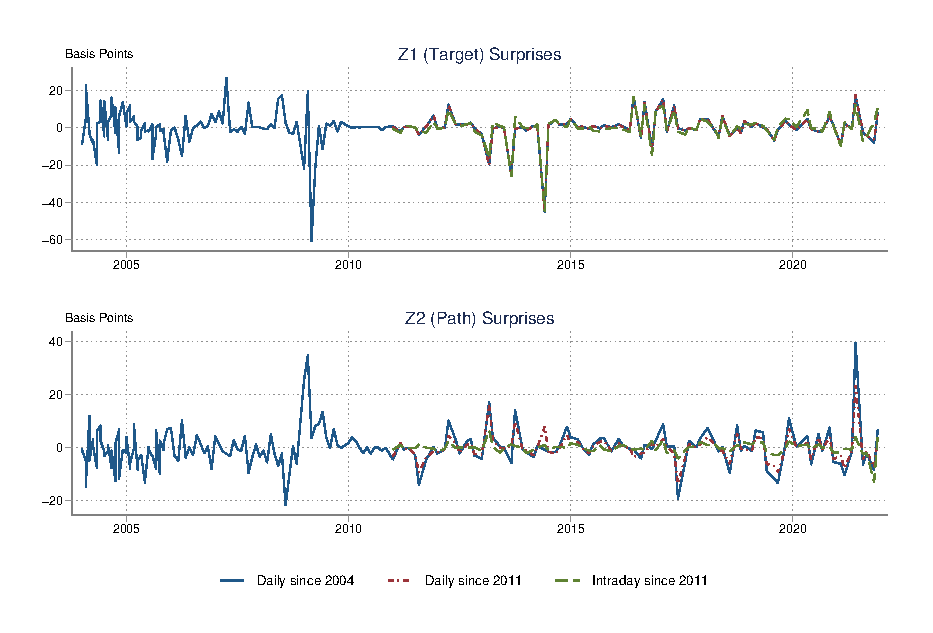
\includegraphics[width=1\textwidth,height=.4\textheight]{../Figures/factorslines.eps} \\
			\end{center}
			\vspace{-0.4cm}
			\fignotes{This figure compares the evolution of the \( \rtdone \) (target) and \( \rtdtwo \) (path) factors or surprises obtained with daily data since 2004 (solid line) and 2011 (dash-dotted line), and with intraday data since 2011 (dashed line). The sample includes all regular monetary policy announcements up to \lastobs{}.}
		\end{minipage}
	\end{center}
\end{figure}

The figure confirms that two monetary policy factors in Mexico is not a recent phenomenon, in line with table \ref{tab:ranktests}. 
Nevertheless, even though daily data yields longer time series, they have relatively less explanatory power and precision during the estimation \parencite{KearnsManners:2006,Solis:FX}, so the rest of the analysis uses the factors identified with intraday data.


\subsection{Interpreting the Factors} \label{sec:interpretation}
The factors \(\rtdone\) and \(\rtdtwo\) are henceforth referred to as the target and path factors or surprises. 
By definition, \(\rtdone\) moves one-to-one with changes in the 3-month swap. 
Thus, \(\rtdone\) can be related to surprises in the \textit{current} policy rate, since changes in the 3-month swap adequately capture the monetary stance in the short run \parencite{Solis:FX}. 
On the other hand, \(\rtdtwo\) is aligned with movements in the 12-month swap that are unrelated to changes in the 3-month swap, so the second factor could in principle just capture movements in long-term yields.\footnote{ By construction, \(\rtdone\) is essentially the same as the policy rate surprises in \textcite{Solis:FX}, the correlation between the two measures is \(0.99\). Meanwhile, the correlation between \(\rtdtwo\) and the residual of a regression of the change in the 12-month swap on the change in the 3-month swap is \(0.98\).} 
The evidence in figure \ref{fig:factorspoints} and table \ref{tab:statements} below, however, supports its association with surprises about the \textit{future} path of the policy rate.\footnote{\textcite{GSS:2005a,Swanson:2021} show that the first and second factors in the U.S. also relate to surprises about the policy rate and its future path communicated via statements, respectively.} 
More broadly, path surprises by emerging market central banks could be considered as communication surprises or as a subtle form of forward guidance. 

Figure \ref{fig:factorspoints} plots the estimated target and path surprises for relevant dates over the sample period. 
Target surprises are in the horizontal axis, and path surprises are in the vertical axis; the units are basis points. 
The figure is obtained by leaving out the points inside an arbitrary radius.\footnote{Target and path surprises are orthogonal to each other by construction, so no correlation is to be expected between the dots in the figure.} 
A positive value in any of the two surprises represents a tightening in the monetary stance, and a negative value represents an easing. 
Accordingly, the first quadrant shows announcements with target and path tightening surprises, while the third quadrant shows dates in which both surprises eased; 
in the second and fourth quadrants, one surprise tightened and the other eased.
Notice that Banxico has used all four possible combinations of target and path surprises. 

\begin{figure}[t]
	\caption{Monetary Policy Dimensions} \label{fig:factorspoints}
	\begin{center}
		\begin{minipage}{0.9\linewidth}
			\begin{center}
				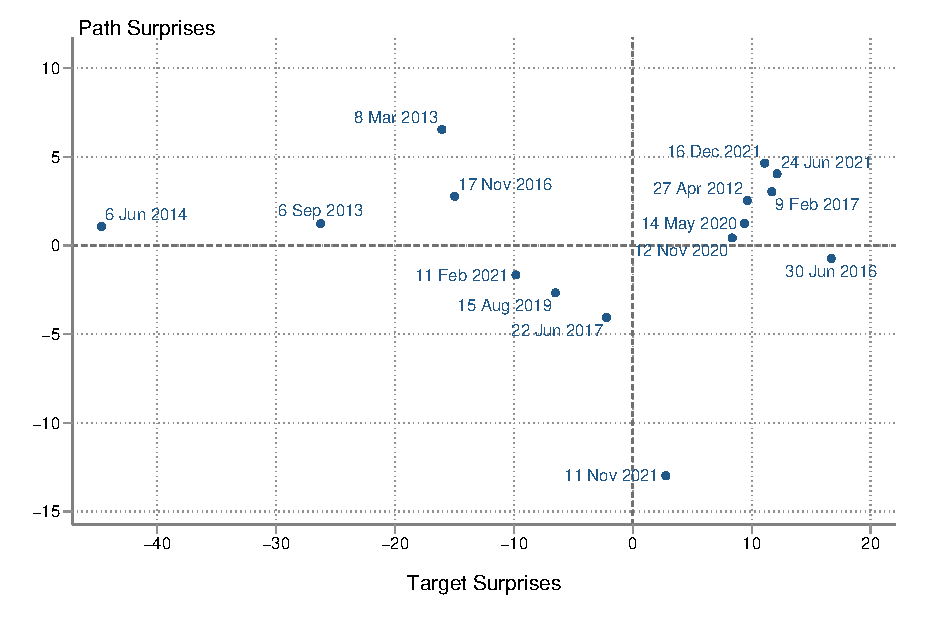
\includegraphics[width=1\textwidth,height=.4\textheight]{../Figures/factorspointstg.eps} \\
			\end{center}
			\vspace{-0.4cm}
			\fignotes{This figure plots the largest intraday target and path surprises (expressed in basis points) between January 2011 and \lastobsflwbdm, as explained in the main text.} 
		\end{minipage}
	\end{center}
\end{figure}


\subsubsection{Statements and Path Surprises} \label{sec:pathsurprises}
Central banks can use statements to influence expectations about future monetary policy decisions and to reduce policy uncertainty. This part shows that Banxico communicates information about the future path of its policy rate via statements. 

Table \ref{tab:statements} shows that path surprises are closely related to information in the statements. 
It contains excerpts of statements for days in which path surprises are large in absolute value (most of them plotted in figure \ref{fig:factorspoints}). 
All the excerpts contain clear references to the monetary stance outlook, and several of them make explicit reference to the future path of the policy rate. See, for instance, the excerpts for March 2013, June 2017, May and June 2022, February and March 2023.\footnote{The link between statements and path surprises predates the start of the intraday sample in 2011. For instance, the largest path \textit{tightening} surprise pre-2011 (using daily data) occurred on June 2009 along with a statement indicating that `the Board considers that its easing cycle is close to an end'.} 
Notice that the text and the signs of the path surprises are consistent with each other, which is noteworthy since no textual analysis is involved in the identification of the surprises. 

\afterpage{
	\begin{normalsize}
		\begin{landscape}
			\begin{table}
				\centering
				\caption{Summary of Statements in Selected Dates}
				\label{tab:statements}
				\begin{tabular}{p{2.4cm}S[table-format=2.2]S[table-format=2.2]p{17.4cm}p{2.4cm}S[table-format=2.2]S[table-format=2.2]p{17.4cm}p{2.4cm}S[table-format=2.2]S[table-format=2.2]p{17.4cm}p{2.4cm}S[table-format=2.2]S[table-format=2.2]p{17.4cm}}
					\toprule
					\multicolumn{1}{c}{Date} & \multicolumn{1}{c}{Target} & \multicolumn{1}{c}{Path} & \multicolumn{1}{c}{Description} \\
					\midrule
					Jun 23, 2022 &   7.41 & -14.93 & Statement notes that the Board `will assess to act with the same forcefulness if required,' after increasing the policy rate by 75 basis points for the first time ever. \\
					Mar 8, 2013 & -15.64 &  11.77 & Statement makes clear that the 50 basis point cut in the policy rate `does not represent the beginning of an easing cycle.' \\
					Feb 9, 2023 &  18.17 &  11.45 & Statement indicates that `the next increase in the policy rate may be of a smaller magnitude,' after 14 consecutive increases amounting to 7\%. \\
					Dec 16, 2021 &   9.42 &  10.52 & Statement highlights that the forecasts for headline and core inflation were revised upwards `again, especially those for 2022,' and that the balance of risks for inflation `has deteriorated again.' \\
					Mar 30, 2023 &  -2.14 &  -8.53 & Statement notes that inflation `has fallen more than expected,' and removes `the next increase in the policy rate may be of a smaller magnitude' from the previous statement. \\
					Jun 22, 2017 &  -2.07 &  -8.03 & Statement drops reference to do `the necessary tightenings ahead' from the previous statement. \\
					Aug 15, 2019 &  -6.05 &  -5.82 & Statement notes that `inflation decreased as expected,' while `the negative output gap widened more than expected.' \\
					May 12, 2022 &   0.85 &   5.78 & Statement highlights that inflation reached `its highest level since January 2001,' so the Board `will consider to act more forcefully,' following four increases of 25 and four of 50 basis points. \\
					Aug 12, 2021 &  -6.94 &  -5.45 & Statement notes that although the expected path of inflation increased, inflation is `expected to decrease, especially for horizons longer than one year.' \\
					Nov 11, 2021 &  -7.61 &  -5.24 & Statement indicates that the shocks to inflation are considered to be `mainly' transitory. \\
					\bottomrule
				\end{tabular}
			\end{table}
		\end{landscape}
	\end{normalsize}
}

The tightening cycle that started in mid-2016 further exemplifies the link between path surprises and statements. 
The 2016 U.S. presidential election generated uncertainty about the bilateral relation of the two countries. Between early-November 2016 and mid-January 2017, the peso depreciated by more than 14\%. 
In addition, the Mexican government raised the minimum wage and ended gasoline subsidies in early-2017. By mid-2017, inflation had risen for 10 consecutive months. 
In that context, Banxico raised its policy rate by 50 basis points on June and September 2016, more than the market expected according to surveys, followed by six more consecutive tightenings (three of 50 and three of 25 basis points) to contain the rising inflation risks. 
In the statement for the last hike on June 22, 2017, Banxico dropped the reference to do `the necessary tightenings ahead' from the previous statement. 
The hike was largely anticipated by the market (i.e., a small target surprise), but the wording of the statement suggested the end of the tightening cycle, delivering the largest path easing surprise at the time. 

Statements have also been used to contain path surprises. 
Contrary to survey expectations of no change in the policy rate, on June 6, 2014, Banxico cut the rate by 50 basis points, but in the statement indicated that `no further reductions in the policy rate are expected in the foreseeable future.' Therefore, the policy rate was cut unexpectedly, but the statement portrayed the decision as a one-off cut. 

In sum, target and path surprises respectively capture unanticipated changes in the policy rate and news about its future path communicated via statements. 


\section{The Effects of Monetary Policy on Asset Prices} \label{sec:assets}
The previous section shows that target and path surprises capture news about the policy rate and its future path. 
This section quantifies how the exchange rate and the yield curve respond to the surprises. 
The next section studies the response of portfolio flows.


\subsection{Contemporaneous Effects}
The following event-study regression measures the on-impact effects of the two types of monetary policy surprises on the exchange rate and the yield curve:
\begin{equation} \label{eq:nTwoFacP}
	\eqTwoFacP ,
\end{equation}
\noindent in which \(\depvar\) denotes the intraday exchange rate returns or the intraday changes in bond yields, \(\rtdonereg\) and \(\rtdtworeg\) are the intraday surprises in the policy rate and its future path, and \(\errorreg\) is the error term. 
All the variables are expressed in basis points. 
The standard errors are computed using 10,000 bootstrap simulations given that \(\rtdonereg\) and \(\rtdtworeg\) are generated regressors \parencite[see][Appendix B]{Swanson:2021}.\footnote{The statistical significance of the results is essentially the same whether bootstrapped or asymptotic standard errors are used.}

The parameters of interest are \(\slopetrgt\) and \(\slopepath\), they measure the response of the exchange rate and bond yields to the two types of surprises. A monetary policy tightening should appreciate the currency, according to standard open economy models, and increase bond yields at different maturities, due to increases in interest rate expectations and term premia. In this sense, \(\slopetrgt\) and \(\slopepath\) are expected to be negative for the exchange rate (since it is expressed in pesos per dollar) and positive for bond yields.

Table \ref{tab:fctrsfxyc} reports the results of the estimation. The first column for each dependent variable shows the coefficient estimates when they are regressed only on target surprises, and the second column adds path surprises as a regressor. 
The first columns align with the results using policy rate surprises in \textcite{Solis:FX}.

\afterpage{
	\begin{normalsize}
		\begin{landscape}
			\begin{table}
				\begin{center}
					\caption{The Response of Asset Prices to Target and Path Surprises} \label{tab:fctrsfxyc} %: Intraday Data
					\begin{threeparttable}
						\begin{tabularx}{0.95\linewidth}{l*{10}C}
							\toprule
							&\multicolumn{2}{c}{FX Returns} & \multicolumn{2}{c}{\(\Delta\) 2Y Yield} & \multicolumn{2}{c}{\(\Delta\) 5Y Yield} & \multicolumn{2}{c}{\(\Delta\) 10Y Yield} & \multicolumn{2}{c}{\(\Delta\) 30Y Yield}\\
							\cmidrule(lr){2-3}\cmidrule(lr){4-5}\cmidrule(lr){6-7}\cmidrule(lr){8-9}\cmidrule(lr){10-11}
							Target & -2.54*** & -2.54*** & 0.74*** & 0.74*** & 0.54*** & 0.47*** & 0.46*** & 0.46*** & 0.31*** & 0.31***\\
							& (0.39) & (0.39) & (0.05) & (0.04) & (0.06) & (0.05) & (0.05) & (0.04) & (0.05) & (0.04)\\
							Path &  & -1.36* &  & 0.43*** &  & 0.57*** &  & 0.44*** &  & 0.41***\\
							&  & (0.75) &  & (0.09) &  & (0.1) &  & (0.08) &  & (0.08)\\
							\midrule
							Obs. & 99 & 99 & 83 & 83 & 64 & 64 & 83 & 83 & 83 & 83\\
							\(R^{2}\) & 0.3 & 0.31 & 0.75 & 0.81 & 0.4 & 0.62 & 0.56 & 0.7 & 0.37 & 0.54\\
							\bottomrule
							\addlinespace[.75ex]
						\end{tabularx}
						\tabnote{The first column for each dependent variable shows the coefficient estimates in regressions of intraday yield changes or exchange rate (FX) returns on target surprises; the second column adds path surprises as a regressor. Target and path surprises are obtained from intraday data, as explained in the main text. Intraday changes are calculated starting 10 minutes before to 20 minutes after a monetary policy announcement. The sample includes all regular monetary policy announcements starting on January 2011 for the exchange rate, on January 2013 for 2- 10- and 30-year yields, and on December 2014 for 5-year yields; the sample ends on \lastobs{} in all cases. Figures are expressed in basis points. All regressions include a constant. Bootstrapped standard errors in parentheses. *, **, *** asterisks respectively indicate significance at the 10\%, 5\% and 1\% level.}
					\end{threeparttable}
				\end{center}
			\end{table}
		\end{landscape}
	\end{normalsize}
}

The exchange rate responds to both target and path surprises. A tightening in either surprise appreciates the currency. A 25 basis point (bp) target tightening surprise would appreciate the currency by more than 0.6\%, on average, while an equivalent-size path surprise has almost half the effect, it would appreciate the currency by more than 0.3\%, on average. 
These results are in line with the evidence for the currencies of advanced economies before the global financial crisis \parencite{Rosa:2011JBF}. 

The yield curve also responds to both surprises. 
A tightening in either surprise flattens the yield curve. 
Importantly, path surprises tend to have a stronger effect on medium- and long-term yields and explain a large share of their variability, as seen by comparing the \(R^2\) with one and two regressors, which is consistent with the evidence for the U.S. when its policy rate was not constrained by the zero lower bound \parencite{GSS:2005a,Swanson:2021}. 
However, the influence of Banxico's surprises on the yield curve in Mexico seems to be larger relative to the effect that U.S. surprises have on the U.S. yield curve.\footnote{Comparing the estimates in table \ref{tab:fctrsfxyc} against those in \textcite{GSS:2005a}, on average, a 25 bp target tightening surprise in Mexico vs the U.S. raises the 2- 5- and 10-year yields by 19 vs 12, 12 vs 7, 12 vs 3 bp; while a 10 bp path tightening surprise raises them by 4 vs 4, 6 vs 4, 4 vs 3 bp, respectively.}
This result reflects two non-mutually-exclusive channels according to the expectations hypothesis.\footnote{Since prices are flexible in the long run, long-term expected real interest rates would not be affected.} 
First, it is likely that long-term inflation expectations in Mexico are \textit{less} firmly anchored than in the U.S. \parencites[][fig. 12]{AndreasenChristensenRiddell:2021}[][fig. 10]{Beauregard_etal:2021}. 
Second, monetary policy surprises in Mexico may have a larger effect on the term premium.\footnote{This channel could be explained by reach-for-yield investors who, for instance, switch to long-term bonds in search of higher returns after a target easing, lowering their yields \parencite{HansonStein:2015}.} 
Future research can provide more evidence on both channels.


\subsection{The Changing Impact of Monetary Policy} \label{sec:sbreaksfxyc}

To analyze whether the sensitivity of the exchange rate and bond yields to monetary policy surprises changed over the sample period, I test for a structural break in equation (\ref{eq:nTwoFacP}) using the test developed by \textcite{BaiPerron:2003}, as in \textcite{FerrariKearnsSchrimpf:2021}. This test will also be useful for the analysis of portfolio flows in section \ref{sec:persistenceflows}.\footnote{I thank an anonymous reviewer for highlighting the possibility of structural breaks in portfolio flows.} 

\begin{normalsize}
	\begin{table}
		\begin{center}
			\caption{Structural Break Tests for Asset Prices} \label{tab:sbreaksfxyc} 
			\begin{threeparttable}
				\begin{tabularx}{0.95\linewidth}{l*{6}C}
					\toprule
					                    &  FX         &    2Y Yield         &    5Y Yield         &   10Y Yield         &   30Y Yield         \\
					\cmidrule(lr){2-6}
					Test Statistic           &       27.99         &        4.07         &        9.03         &        7.10         &        8.86         \\
					1\% Crit. Value  &        7.68         &        7.68         &        7.68         &        7.68         &        7.68         \\
					5\% Crit. Value  &        5.74         &        5.74         &        5.74         &        5.74         &        5.74         \\
					10\% Crit. Value &        4.91         &        4.91         &        4.91         &        4.91         &        4.91         \\
					Break Date          &    10/31/14         &    04/30/15         &    02/07/19         &    04/30/15         &    03/26/15         \\
					Obs.                &          99         &          83         &          64         &          83         &          83         \\
					\bottomrule
					\addlinespace[.75ex]
				\end{tabularx}
				\tabnote{This table reports the results of the structural break test by \textcite{BaiPerron:2003} to assess whether the effect of monetary policy on asset prices has changed over time. The null hypothesis of no structural break in the estimated coefficients \(\beta^{1}_{\idxh}\) and \(\beta^{2}_{\idxh}\) is tested for equation (\ref{eq:nTwoFacP}). The sample starts on January 2011 and ends on \lastobsflwbdm. The format of the dates is Month/Day/Year.}
			\end{threeparttable}
		\end{center}
	\end{table}
\end{normalsize}

Table \ref{tab:sbreaksfxyc} reports the results. For the exchange rate, the test strongly rejects the null hypothesis of no structural break, and identifies \breakdatefx as the date. For bond yields, the test suggests a break in early 2015 for three out of the four yields, although for the 2-year yield it is not significant. I cannot test for a structural break in early 2015 for the 5-year yield because its first observation occurs on December 2014. To simplify the analysis, I use the same date for all yields. Specifically, the one estimated for the 10-year yield on \breakdateyc  (although the results are robust to choosing the date for the 30-year yield on March 26, 2015). Both break dates comprise a period of declining oil prices and uncertainty about the end of the zero lower bound era in the U.S. Table \ref{tab:fctrsfxycsb} reports the results of estimating equation (\ref{eq:nTwoFacP}) before (first column) and after (second column) the respective break dates; the results for the 5-year yield are essentially the same as the ones in table \ref{tab:fctrsfxyc} and thus not reported. 

\afterpage{
	\begin{normalsize}
		\begin{landscape}
			\begin{table}
				\begin{center}
					\caption{The Response of Asset Prices to Target and Path Surprises Before and After Break Dates} \label{tab:fctrsfxycsb} %: Intraday Data
					\begin{threeparttable}
						\begin{tabularx}{0.95\linewidth}{l*{8}C}
							\toprule
							                    &\multicolumn{2}{c}{FX Returns} &\multicolumn{2}{c}{\(\Delta\) 2Y Yield}&\multicolumn{2}{c}{\(\Delta\) 10Y Yield}&\multicolumn{2}{c}{\(\Delta\) 30Y Yield}\\\cmidrule(lr){2-3}\cmidrule(lr){4-5}\cmidrule(lr){6-7}\cmidrule(lr){8-9}
							Target              &       -1.61***&       -5.36***&        0.88***&        0.64***&        0.61***&        0.32***&        0.49***&        0.16** \\
							&      (0.39)   &      (0.77)   &     (0.059)   &     (0.083)   &     (0.052)   &     (0.064)   &     (0.042)   &     (0.071)   \\
							Path                &       -5.24***&        1.23   &        0.70***&        0.44***&        0.68***&        0.49***&        0.71***&        0.45***\\
							&      (1.52)   &      (0.92)   &      (0.17)   &      (0.11)   &      (0.19)   &     (0.087)   &      (0.13)   &     (0.094)   \\\midrule
							Obs.                &          30   &          69   &          18   &          65   &          18   &          65   &          18   &          65   \\
							\(R^{2}\)           &        0.48   &        0.61   &        0.96   &        0.71   &        0.92   &        0.60   &        0.91   &        0.44   \\
							\bottomrule
							\addlinespace[.75ex]
						\end{tabularx}
						\tabnote{The first column for each dependent variable shows the coefficient estimates in regressions of intraday yield changes or exchange rate (FX) returns on target and path surprises \textit{before} the respective break date; the second column reports the coefficient estimates \textit{after} the break date. Target and path surprises are obtained from intraday data, as explained in the main text. Intraday changes are calculated starting 10 minutes before to 20 minutes after a monetary policy announcement. The sample includes all regular monetary policy announcements starting on January 2011 for the exchange rate, on January 2013 for 2- 10- and 30-year yields; the sample ends on \lastobs{} in all cases. The break date for the exchange rate is \breakdatefx{} and for bond yields is \breakdateyc. Figures are expressed in basis points. All regressions include a constant. Bootstrapped standard errors in parentheses. *, **, *** asterisks respectively indicate significance at the 10\%, 5\% and 1\% level.}
					\end{threeparttable}
				\end{center}
			\end{table}
		\end{landscape}
	\end{normalsize}
}

The response of the exchange rate is stronger to path surprises before the end of 2014, and to target surprises afterwards.\footnote{Also notice that the explanatory power of the surprises (in terms of \(R^{2}\)) in both subsamples increases considerably relative to the whole sample. These results, as well as those for bond yields in the next paragraph, are robust to using an M-estimator that reduces the impact of outliers.} 
Before end-2014, the effect of path surprises is almost four times larger relative to the whole sample, while for target surprises it lowers by more than a third. 
In contrast, the effect of target surprises more than doubles after end-2014. 
Accordingly, a 25 bp target (post-2014) or path (pre-2014) tightening surprise would appreciate the currency by 1.3\%. 	
The response of the currencies of advanced economies is also stronger after the global financial crisis \parencite{FerrariKearnsSchrimpf:2021}.

The response of the yield curve is particularly stronger before the break date. Although the effects of both surprises remain highly statistically significant before and after the break, they explain considerably more of the variability in yields before the break date (in terms of \(R^2\)), which suggests that monetary policy was the main event for bond yields on announcement days; however, it should be taken with caution given the relatively small sample size before the break date. Finally, notice that path surprises continue to have stronger on-impact effects on long-term yields than target ones in both subsamples. 

The relative role of the surprises for asset prices can thus change over time. The intuition behind these results is discussed in section \ref{sec:persistencefxyc}. 


\subsection{Persistence} \label{sec:persistencefxyc}
Monetary policymakers are not only interested in the initial reaction to the surprises but on how persistent they are. 
This subsection assesses that persistence using local projections following \textcite{Jorda:2005}. Specifically, I run the following regressions: 
\begin{equation} \label{eq:nLPprices}
	\eqLPprices,
\end{equation}
\noindent in which \(\idxh\) indicates the horizon in days with \(\idxh = 0, 1, \ldots, 30\), \(\yld_{\idxsfwd}\) is a bond yield or the log of the exchange rate at the close of day \(\idxsfwd\), \(\rtdonereg\) and \(\rtdtworeg\) are equal to the intraday surprises on announcement days \(\idxt\) and zero otherwise,\footnote{Although the factors are uncorrelated by construction, including them together increases efficiency.} \(\ctrls_{\idxslag}\) is a vector of one-day lagged variables to control for potential drivers of the given assets, and \(u_{\idxsfwd}\) is the error term. 
Since the factors are indeed surprises, no controls are needed,\footnote{In fact, all the results are essentially the same when no controls are included.}  
but they are considered here for comparison with the analysis of portfolio flows in section \ref{sec:persistenceflows} for which it might be more reasonable to include controls. 
All responses are assessed relative to a one basis point tightening of the respective surprise. 
The parameters of interest are \(\beta^{1}_{\idxh}\) and \(\beta^{2}_{\idxh}\), they measure the average response of the dependent variable to the surprises at horizon \(\idxh\).
The 95\% confidence bands are computed using 10,000 bootstrap simulations.

The controls comprise the exchange rate (for the bond yields), the daily returns of the Mexican stock exchange as a measure of local financial conditions, 
the 10-year U.S. Treasury yield from the Federal Reserve’s H.15 dataset to account for global financial conditions, 
the Cboe's volatility index (VIX) as a measure of risk aversion and economic uncertainty, 
the J.P. Morgan Emerging Market Bond Index (EMBI) to capture developments in emerging market sovereign bonds, 
the West Texas Intermediate (WTI) crude oil price as it can influence the exchange rate and bond issuances since Mexico is an oil exporter country, 
the 5-year credit default swap (CDS) for Mexico to account for sovereign default risk, 
the TED spread as an indicator of credit risk in the global financial sector and 
its local version calculated as the difference between the one-month interbank rate (TIIE28D) and the one-month Mexican Treasury bill rate. 
\textcite{CFS:2021} use similar controls in their study of the liquidity premium in the Mexican bond market.

\afterpage{
	\begin{figure}[tbph]
		\caption{Exchange Rate Response to Target and Path Surprises} \label{fig:LPFXsb}
		\begin{center}
			\begin{minipage}{\linewidth}
				\begin{center}
					\begin{subfigure}[b]{0.475\textwidth}
						\centering
						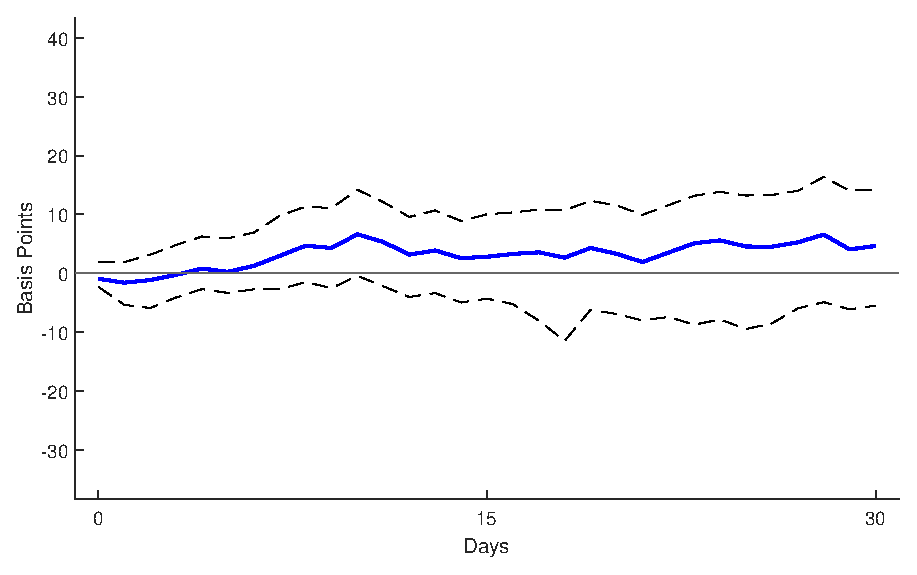
\includegraphics[width=\textwidth]{../Figures/Target11FXpre.eps}
						\caption[]{{\small Target Surprise Pre}} \label{subfig:Target11FXpre}
					\end{subfigure}
					\hfill
					\begin{subfigure}[b]{0.475\textwidth}  
						\centering 
						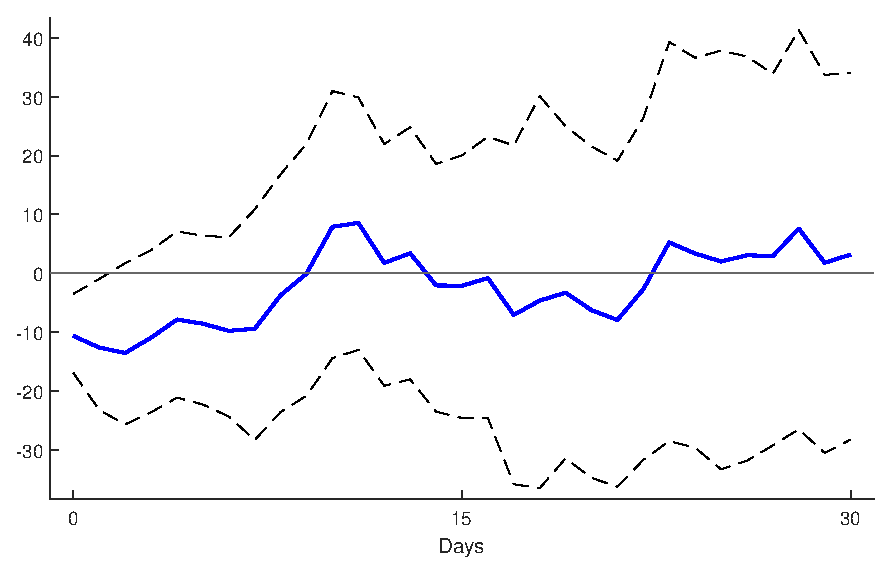
\includegraphics[width=\textwidth]{../Figures/Path11FXpre.eps}
						\caption[]{{\small Path Surprise Pre}} \label{subfig:Path11FXpre}
					\end{subfigure}
					\vskip\baselineskip
					\begin{subfigure}[b]{0.475\textwidth}   
						\centering 
						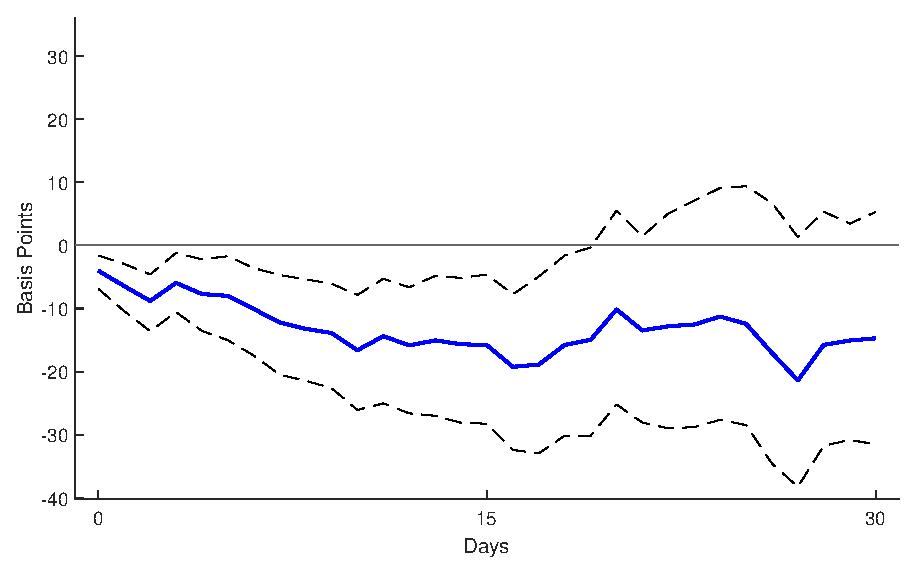
\includegraphics[width=\textwidth]{../Figures/Target11FXpost.eps}
						\caption[]{{\small Target Surprise Post}} \label{subfig:Target11FXpost}
					\end{subfigure}
					\hfill
					\begin{subfigure}[b]{0.475\textwidth}   
						\centering 
						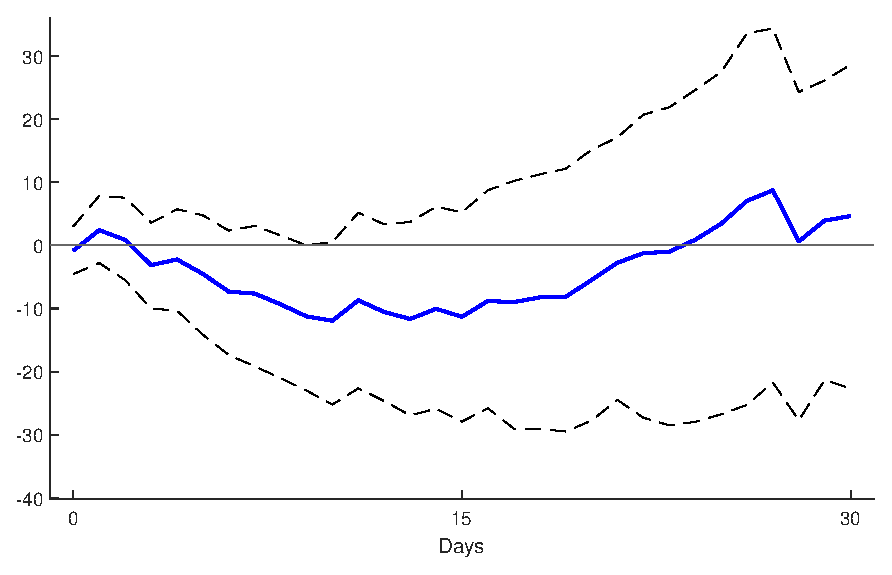
\includegraphics[width=\textwidth]{../Figures/Path11FXpost.eps}
						\caption[]{{\small Path Surprise Post}} \label{subfig:Path11FXpost}
					\end{subfigure}
				\end{center}
				\fignotes{Coefficient estimates for the response of the exchange rate to a 1 basis point target and path tightening surprises from day \(t - 1\) to day \(t + \idxh\), where \(t\) is a day with a monetary policy announcement and \(\idxh = 0, 1, \ldots, 30\). Dashed lines show 95\% bootstrapped confidence bands. The sample starts on January 2011 and ends on \lastobsflwbdm. The top row shows the responses before \breakdatefx, and the bottom row the responses afterwards.}
			\end{minipage} 
		\end{center}
	\end{figure}
}

To discard that the sensitivity of the exchange rate and bond yields to monetary policy identified in section \ref{sec:sbreaksfxyc} is only an on-impact phenomenon, figures \ref{fig:LPFXsb} and \ref{fig:LPYCsb} report the impulse responses before and after their respective break dates.\footnote{Figures \ref{fig:LPFX} and \ref{fig:LPYC} in the appendix report the impulse responses using the whole sample.} 

\afterpage{
	\begin{landscape}
		\begin{figure}[tbph]
			\caption{Yield Curve Response to Target and Path Surprises} \label{fig:LPYCsb}
			\begin{center}
				\begin{minipage}{\linewidth}
					\begin{center}
						\begin{subfigure}[b]{0.475\textwidth}
							\centering
							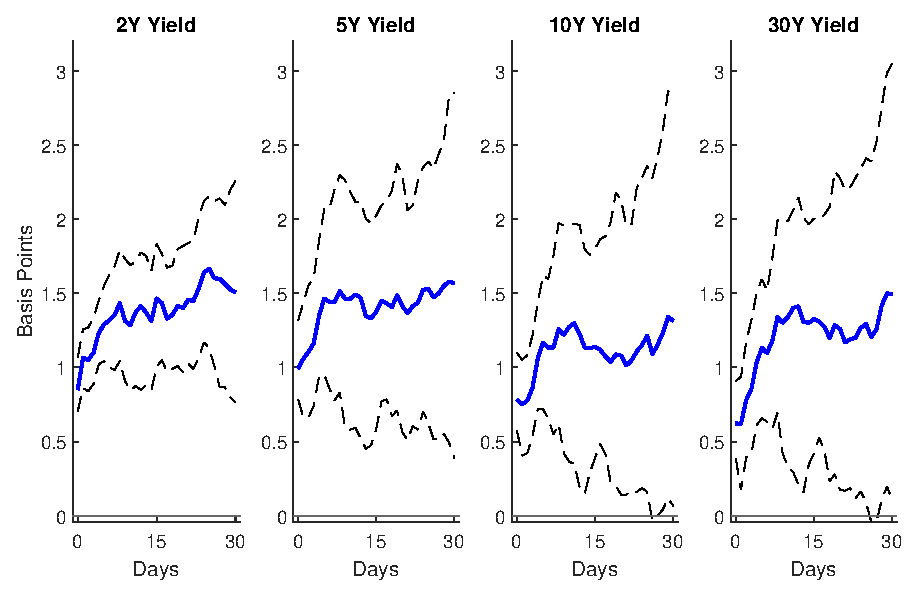
\includegraphics[height=0.35\textheight,width=\textwidth]{../Figures/Target11YCpre.eps}
							\caption[]{{\small Target Surprise Pre}} \label{subfig:Target11YCpre}
						\end{subfigure}
						\hfill
						\begin{subfigure}[b]{0.475\textwidth}  
							\centering 
							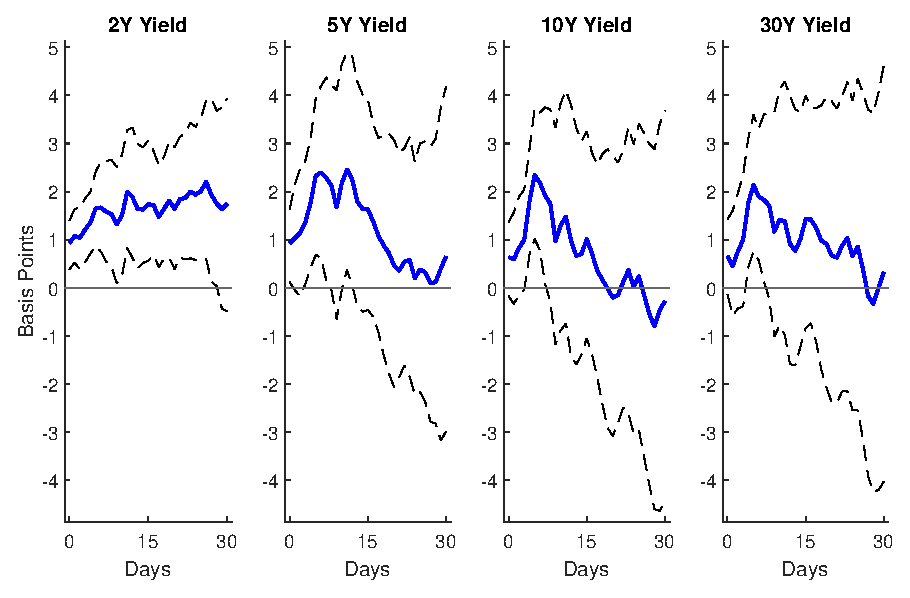
\includegraphics[height=0.35\textheight,width=\textwidth]{../Figures/Path11YCpre.eps}
							\caption[]{{\small Path Surprise Pre}} \label{subfig:Path11YCpre}
						\end{subfigure}
						\vskip\baselineskip
						\begin{subfigure}[b]{0.475\textwidth}   
							\centering 
							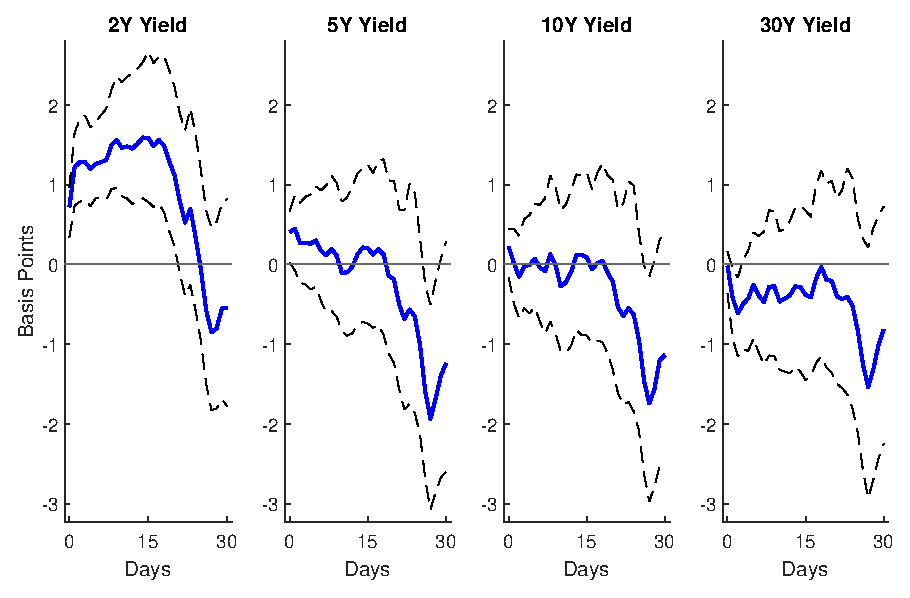
\includegraphics[height=0.35\textheight,width=\textwidth]{../Figures/Target11YCpost.eps}
							\caption[]{{\small Target Surprise Post}} \label{subfig:Target11YCpost}
						\end{subfigure}
						\hfill
						\begin{subfigure}[b]{0.475\textwidth}   
							\centering 
							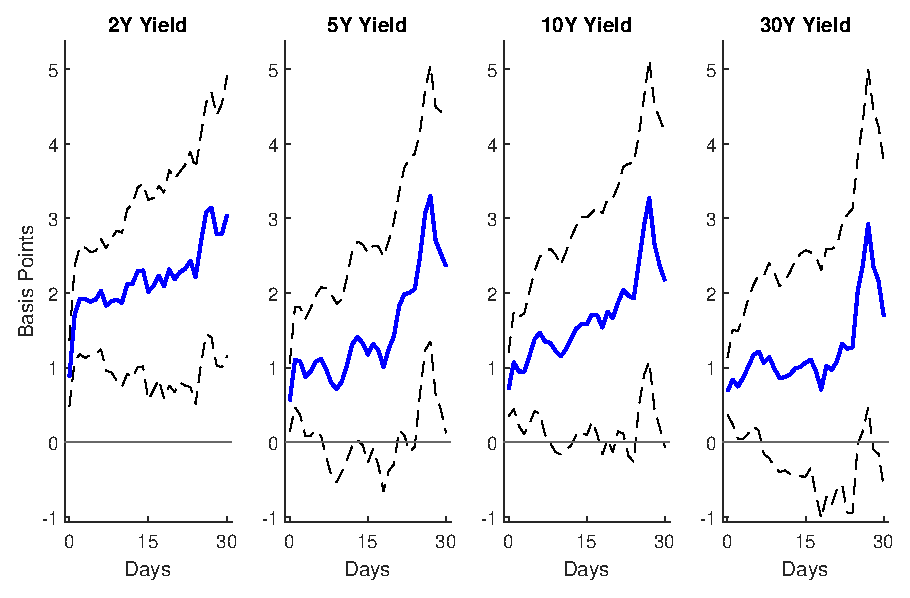
\includegraphics[height=0.35\textheight,width=\textwidth]{../Figures/Path11YCpost.eps}
							\caption[]{{\small Path Surprise Post}} \label{subfig:Path11YCpost}
						\end{subfigure}
					\end{center}
					\fignotes{Coefficient estimates for the response of bond yields to a 1 basis point target and path tightening surprises from day \(t - 1\) to day \(t + \idxh\), where \(t\) is a day with a monetary policy announcement and \(\idxh = 0, 1, \ldots, 30\). Dashed lines show 95\% bootstrapped confidence bands. The sample starts on January 2011 and ends on \lastobsflwbdm. The top row shows the responses before \breakdateyc, and the bottom row the responses afterwards.}
				\end{minipage} 
			\end{center}
		\end{figure}
	\end{landscape}
}

For the exchange rate, the relative importance of the surprises changed, consistent with the results in table \ref{tab:fctrsfxycsb}. 
Before the break, path surprises have a large (10 bp) and persistent effect on the exchange rate for a few days after an announcement, while target surprises have no effect at all.\footnote{That is, the intraday pre-break effect of target surprises in table \ref{tab:fctrsfxycsb} is not detected using daily data. This is consistent with what \textcite{Solis:FX} shows using policy rate surprises.} After the break, the exchange rate only responds to target surprises with an effect that increases over time, reaching almost 20 bp two weeks after an announcement. Without accounting for the break, one would conclude that only path surprises have a persistent effect on the exchange rate (see figure \ref{fig:LPFX} in the appendix).

For bond yields, their response to monetary policy also shifted. 
Before the break, the response to target surprises increases over time (although decreases with maturity), while the response to path surprises is stronger but much less persistent. 
After the break, the response to target surprises is stronger but persistent only for the 2-year yield, while the response to path surprises increases significantly over time for all the yields. 

The break dates of the exchange rate and bond yields are close enough to suggest that forex investors weight target and path surprises differently to bond investors, possibly reflecting their different investment profiles. The frequency of target and path surprises increased post-2014 (see figure \ref{fig:factorslines}).
Before end-2014, the market largely anticipated most policy decisions by Banxico ahead of time.\footnote{With a few exceptions, both surprises tended to be relatively small (within \(\pm\) 5 bp).} 
After end-2014, Banxico has dealt with two inflationary cycles, one after the 2016 U.S. presidential election and some local reforms (see section \ref{sec:pathsurprises}), and the other after the global post-pandemic recovery, during which Banxico has frequently surprised the market.
The nature of the change in figures \ref{fig:LPFXsb} and \ref{fig:LPYCsb} suggests that forex investors give more weight to information about the \textit{future} stance of monetary policy in periods of relative stability, but more weight to \textit{current} monetary policy news when uncertainty increases. Bond investors, on the other hand, seem to give more weight to the future monetary policy outlook under uncertainty. 

In sum, target and path surprises play an important role in the transmission of monetary policy to the exchange rate, a vital channel for open economies, as well as to bond yields which, in particular, can improve the implementation of monetary policy, to the extent that medium- and long-term yields influence the spending decisions of households and firms. 
Moreover, their effects on asset prices are persistent, lasting days after an announcement. 
This delayed response aligns with a slow-moving capital explanation \parencite{Duffie:2010}, in which big players like pension funds and foreign investors take time to respond to the surprises. 
The evidence in the next section supports this interpretation. 


\section{The Effects of Monetary Policy on Portfolio Flows} \label{sec:flows}
This section shows that domestic and foreign investors rebalance their debt portfolios in response to target and path surprises. The analysis exploits the availability of daily data to better understand the transmission mechanisms of monetary policy. 

\subsection{Daily Data on Portfolio Flows} \label{sec:flowsdaily}
Banxico collects daily data on the value of the holdings of different types of Mexican government securities, including Treasury bills (cetes), fixed-rate bonds (bonos) and inflation-protected bonds (udibonos). 
The analysis focuses on cetes and bonos because they are related to the (nominal) yield curve. The appendix reports the results for udibonos.

Banxico reports the holdings of domestic and foreign investors. 
Figure \ref{fig:frgvsdomctsbnd} in the appendix compares the level of cetes and bonos holdings by residence. 
Foreign investors were once the main players in the cetes and bonos markets. They increased their bonos holdings substantially since they were included in the Citigroup's World Government Bond Index in 2010 \parencite{Banxico:2014} and up to 2020,\footnote{This trend increased the liquidity premium in the bonos market \parencite{CFS:2021}.} when they reduced their exposure in response to the Covid-19 pandemic. 
Between late 2012 and early 2016, foreigners were also the main holders of cetes but rising hedging costs after the end of the zero lower bound era in the U.S. made the short-term carry trade less attractive, which partly explains the decline since then. 

Banxico categorizes domestic investors into banks, mutual funds, pension funds, insurers and non-financial investors (firms and households). 
Figures \ref{fig:categscts} and \ref{fig:categsbnd} in the appendix show the level of cetes and bonos holdings by domestic investors, respectively. 
In the cetes market, non-financial investors are key players, while pension funds increased their holdings around the time foreign investors retreated, and mutual funds\footnote{In Mexico, most mutual funds are shot-term debt funds with highly liquid investments.} 
have increased their holdings recently. 
In the bonos market, pension funds are key players but, in recent years, non-financial investors and banks started accumulating a larger share of bonos. 
Insurers play a minor role in both markets and are thus no longer considered.

Daily portfolio flows are defined as the daily change in the holdings. 
Positive and negative values respectively indicate purchases and sales of the security.
The flows are expressed in billions of pesos. The bonos holdings are adjusted for valuation effects before computing their flows. Table \ref{tab:summflowsdy} in the appendix summarizes the flow data. 

To account for the fact that changes in the nominal value of bonos holdings can reflect either a change in the amount of bonos or a change in the value of the bonos, I deflate the nominal value of bonos holdings with a rate equal to the percentage change in the price, so that a change in the holdings reflects net purchases, regardless of price movements.
The daily percentage change in the price of the bonos is approximated as minus the duration times the daily change in the yield. 
The duration of the bonos is calculated using the par yields from the Bloomberg Fair Value (BFV) curve for Mexico and the average maturity of the bonos reported by Banxico.\footnote{The change in the log price of the bond, \(\mathrm{d}\log (P)\), is approximately equal to \(- D_{mod} \times \mathrm{d} y\), in which \(D_{mod}\) is the modified duration and \(\mathrm{d} y\) is the change in the yield. Each day, the BFV yield closest to the average maturity is used to calculate \(D_{mod}\) and \(\mathrm{d} y\). Banxico reports every month the average maturity (expressed in days) of the bonos outstanding. For the adjustment, the average maturity is expressed in years and rounded to the nearest integer; the same value is used for all the days in a month.} 
Although the adjustment is far from perfect, it is reasonable given the available data (e.g., average maturity is not broken down by tenor or by type of investor). 
The results are robust to the adjustment.


\subsection{The Response of Portfolio Flows} \label{sec:persistenceflows}
Given the evidence in section \ref{sec:persistencefxyc} of a delayed response in asset prices, the analysis focuses on the persistence (rather than on the contemporaneous effects) using local projections. 
Specifically, I run the following regressions:
\begin{equation} \label{eq:nLPflows}
	\eqLPflows,
\end{equation}	
\noindent in which, the dependent variable \(\hld_{\idxsfwd}\) equals the holdings of a given category on day \(\idxsfwd\),
and the vector of one-day lagged variables \(\ctrls_{\idxslag}\) controls for potential drivers of the flows (using the same controls as before).\footnote{The coefficient \(\alpha^{2}_{\idxh}\) is virtually one in the estimations, so equation (\ref{eq:nLPflows}) is essentially a regression of the flows (\(\hld_{\idxsfwd} - \hld_{\idxslag}\)) on the surprises and the controls.}  
The rest is equal to the case with asset prices in equation (\ref{eq:nLPprices}). 
The analysis below focuses on the responses of domestic and foreign investors in cetes and bonos. Figures \ref{fig:LPUdibonosCateg1} to \ref{fig:LPUdibonosCateg2} in the appendix report the responses for the different categories of domestic investors as well as for udibonos.

Notice that, given the nature of the data, non-significant results are likely but can still be informative. Even though the holding categories classify investors by type, they are still broad enough to bring together a heterogeneous group of investors. For instance, banks (one of the categories of domestic investors) puts together the big banks along with niche banks and others, not all of which will respond in the same direction to a monetary policy surprise. Such varied responses will reflect in wide confidence bands, which can be indicative of a portfolio rebalancing effect, not a homogeneous one in which the investors in a category respond on average in the same direction, but a heterogeneous one within and across sectors. In this sense, statistically significant results are especially meaningful.

\afterpage{
	\begin{figure}[tbph]
		\caption{Cetes Flow Response to Target and Path Surprises by Investor Residence} \label{fig:LPCetesCateg1sb}
		\begin{center}
			\begin{minipage}{\linewidth}
				\begin{center}
					\begin{subfigure}[b]{0.475\textwidth}
						\centering
						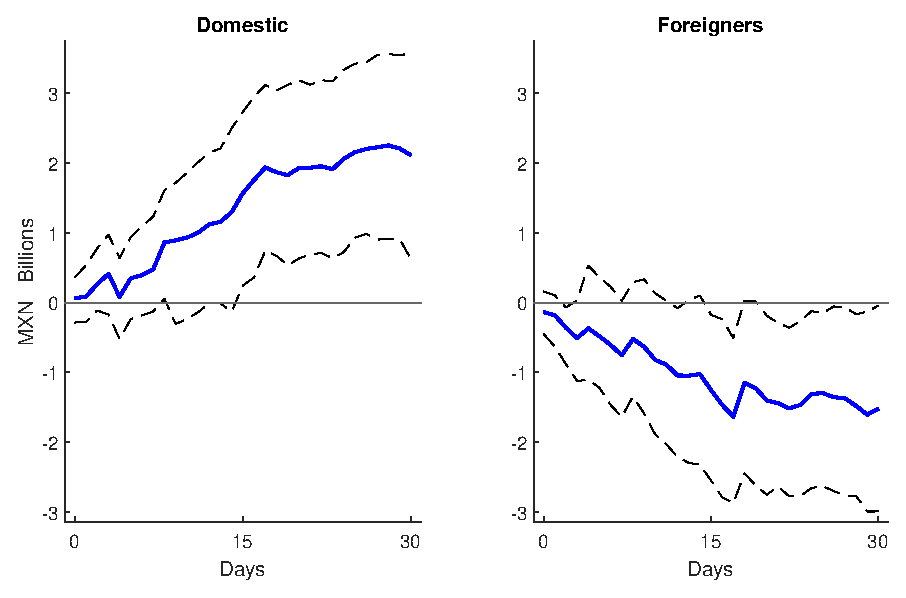
\includegraphics[width=\textwidth]{../Figures/Target11CetesCateg1pre.eps}
						\caption[]{{\small Target Surprise Pre}} \label{subfig:Target11CetesCateg1pre}
					\end{subfigure}
					\hfill
					\begin{subfigure}[b]{0.475\textwidth}  
						\centering 
						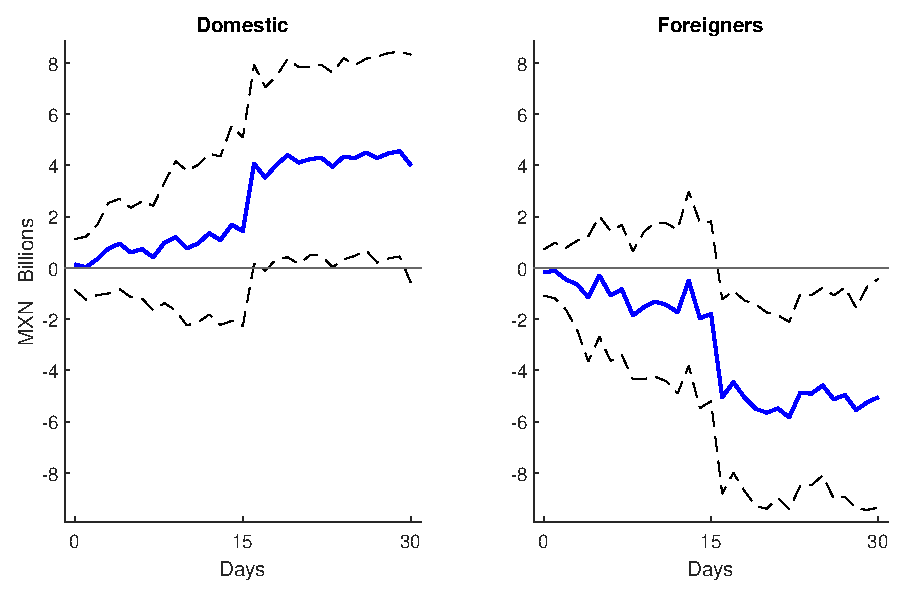
\includegraphics[width=\textwidth]{../Figures/Path11CetesCateg1pre.eps}
						\caption[]{{\small Path Surprise Pre}} \label{subfig:Path11CetesCateg1pre}
					\end{subfigure}
					\vskip\baselineskip
					\begin{subfigure}[b]{0.475\textwidth}   
						\centering 
						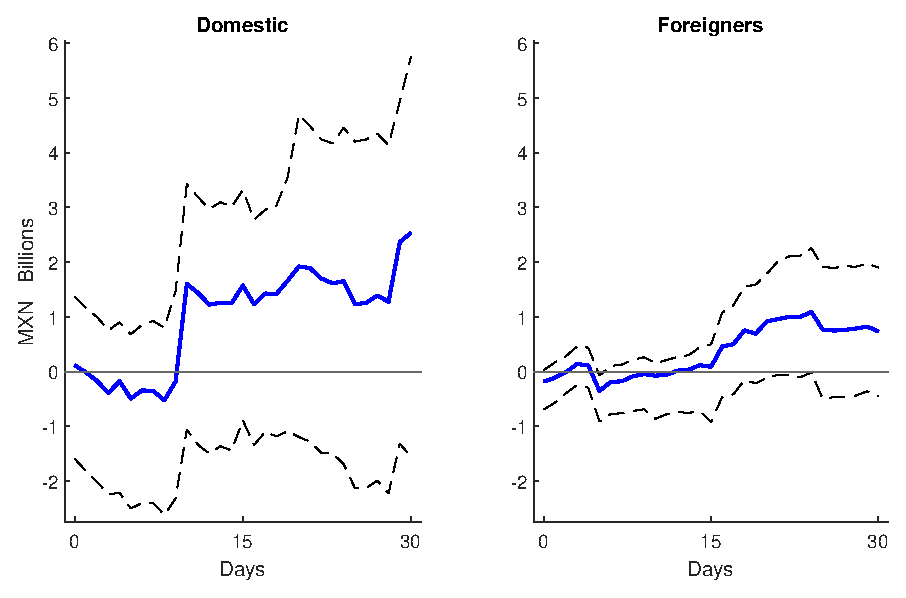
\includegraphics[width=\textwidth]{../Figures/Target11CetesCateg1post.eps}
						\caption[]{{\small Target Surprise Post}} \label{subfig:Target11CetesCateg1post}
					\end{subfigure}
					\hfill
					\begin{subfigure}[b]{0.475\textwidth}   
						\centering 
						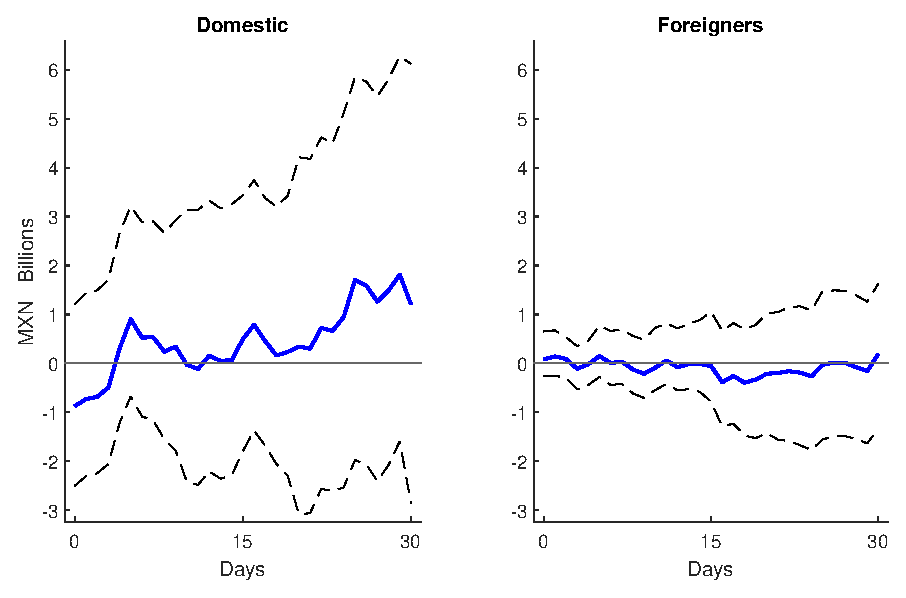
\includegraphics[width=\textwidth]{../Figures/Path11CetesCateg1post.eps}
						\caption[]{{\small Path Surprise Post}} \label{subfig:Path11CetesCateg1post}
					\end{subfigure}
				\end{center}
				\fignotes{Coefficient estimates for the response of cetes flows to a 1 basis point target and path tightening surprises from day \(t - 1\) to day \(t + \idxh\), where \(t\) is a day with a monetary policy announcement and \(\idxh = 0, 1, \ldots, 30\). Dashed lines show 95\% bootstrapped confidence bands. The sample starts on January 2011 and ends on \lastobsflwbdm. The top row shows the responses before \breakdatecetes, and the bottom row the responses afterwards.}
			\end{minipage} 
		\end{center}
	\end{figure}
}

I first test for a structural break using the test developed by \textcite{BaiPerron:2003} again to analyze whether the sensitivity of portfolio flows to monetary policy changed over the sample. Nevertheless, in this case a break is not expected contemporaneously but with a lag given the evidence in section \ref{sec:persistencefxyc}, so I perfom the test for equation (\ref{eq:nLPflows}) at every horizon. Table \ref{tab:sbreaksflows} in the appendix reports the results. I then identify a break date if it is statistically significant and detected for at least three horizons. 
Based on these criteria, there is a break date for foreign investors in cetes on \breakdatecetes, and for domestic investors in bonos on \breakdatebonos, or 2016Q4 and 2021Q1 for ease of reference (see figures \ref{fig:frgvsdomctsbnd} to \ref{fig:categsbnd}). The retreat of foreign investors from the cetes market in 2016 can be explained by the rising hedging costs mentioned in section \ref{sec:flowsdaily}, while the increase in the bonos holdings of domestic investors at the beginning and after the Covid pandemic is likely driven by a flight-to-safety phenomenon.
Figures \ref{fig:LPCetesCateg1sb} and \ref{fig:LPBonosVACateg1sb} show the persistence of cetes and bonos flows before and after their respective break dates.\footnote{Figures \ref{fig:LPCetesCateg1} and \ref{fig:LPBonosVACateg1} in the appendix report the impulse responses using the whole sample.}

The top row of figure \ref{fig:LPCetesCateg1sb} shows the cetes flow response before the break date. 
Before 2016Q4, domestic and foreign investors sit on different sides of the cetes market in response to a tightening of the monetary stance, since their impulse responses virtually mirror each other. In essence, foreigners sold cetes to domestic investors, immediately following a target tightening surprise, and after a couple of weeks following a path tightening surprise. On the domestic side, a key player in this dynamic is the non-financial sector (see the top row of figure \ref{fig:LPCetesCateg2sb}). It is worth noting that this dynamic is only perceived after accounting for the structural break (see figure \ref{fig:LPCetesCateg1}). After 2016Q4, domestic investors increased their positions in cetes to fill the void left in the market by foreigners (see figure \ref{fig:frgvsdomctsbnd}), which suggests that the cetes market is flexible enough to welcome foreign investors when they want to participate and cover for them when they retreat. 

\afterpage{
	\begin{figure}[tbph]
		\caption{Bonos Flow Response to Target and Path Surprises by Investor Residence} \label{fig:LPBonosVACateg1sb}
		\begin{center}
			\begin{minipage}{\linewidth}
				\begin{center}
					\begin{subfigure}[b]{0.475\textwidth}
						\centering
						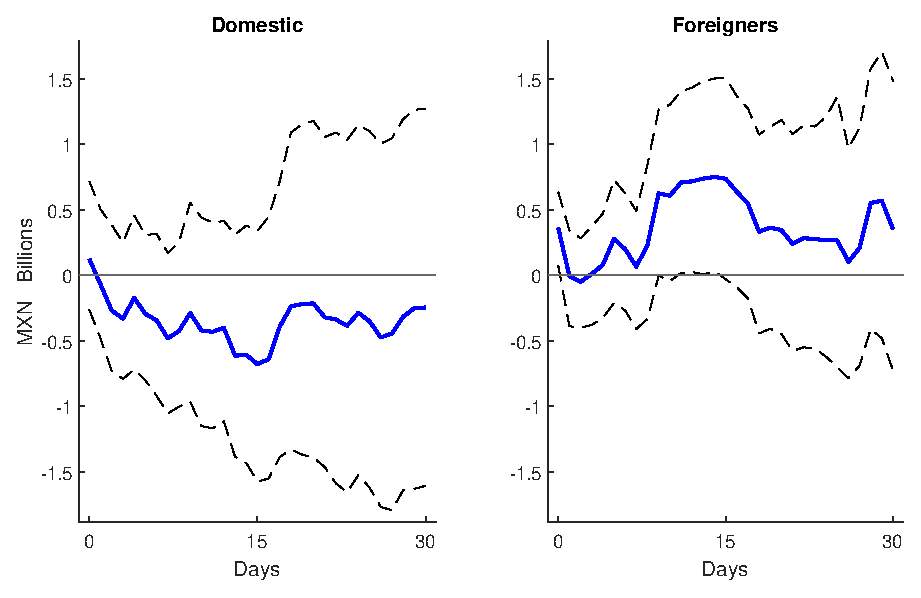
\includegraphics[width=\textwidth]{../Figures/Target11BonosVACateg1pre.eps}
						\caption[]{{\small Target Surprise Pre}} \label{subfig:Target11BonosVACateg1pre}
					\end{subfigure}
					\hfill
					\begin{subfigure}[b]{0.475\textwidth}  
						\centering 
						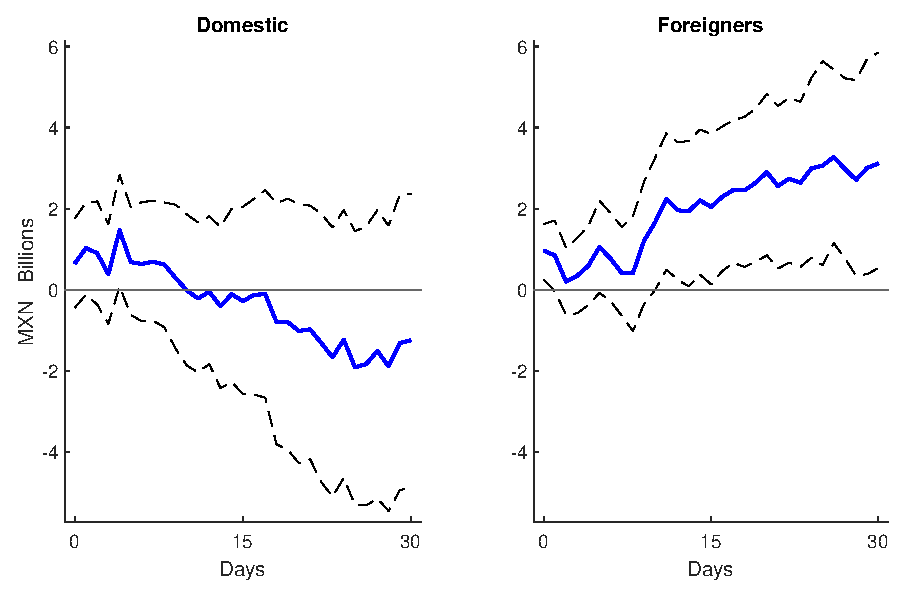
\includegraphics[width=\textwidth]{../Figures/Path11BonosVACateg1pre.eps}
						\caption[]{{\small Path Surprise Pre}} \label{subfig:Path11BonosVACateg1pre}
					\end{subfigure}
					\vskip\baselineskip
					\begin{subfigure}[b]{0.475\textwidth}   
						\centering 
						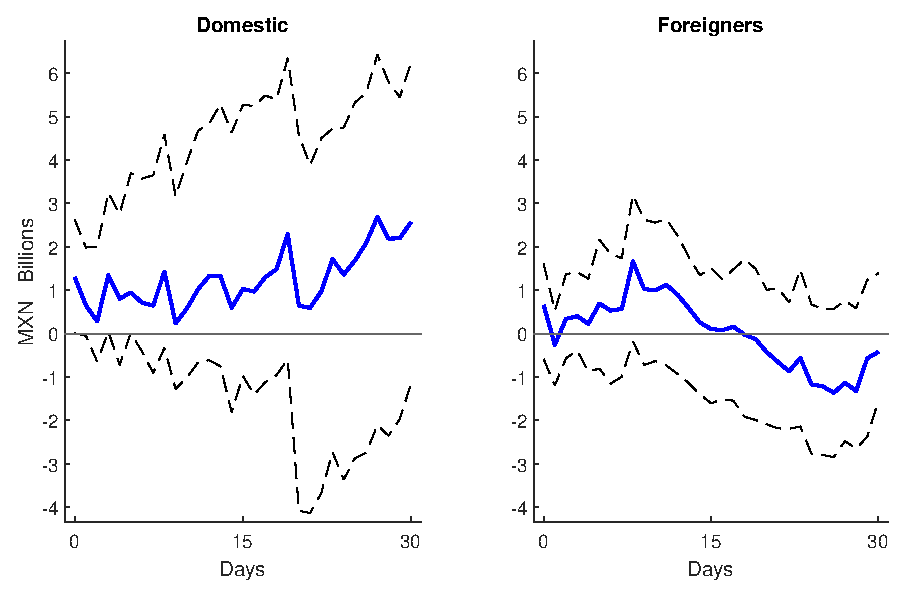
\includegraphics[width=\textwidth]{../Figures/Target11BonosVACateg1post.eps}
						\caption[]{{\small Target Surprise Post}} \label{subfig:Target11BonosVACateg1post}
					\end{subfigure}
					\hfill
					\begin{subfigure}[b]{0.475\textwidth}   
						\centering 
						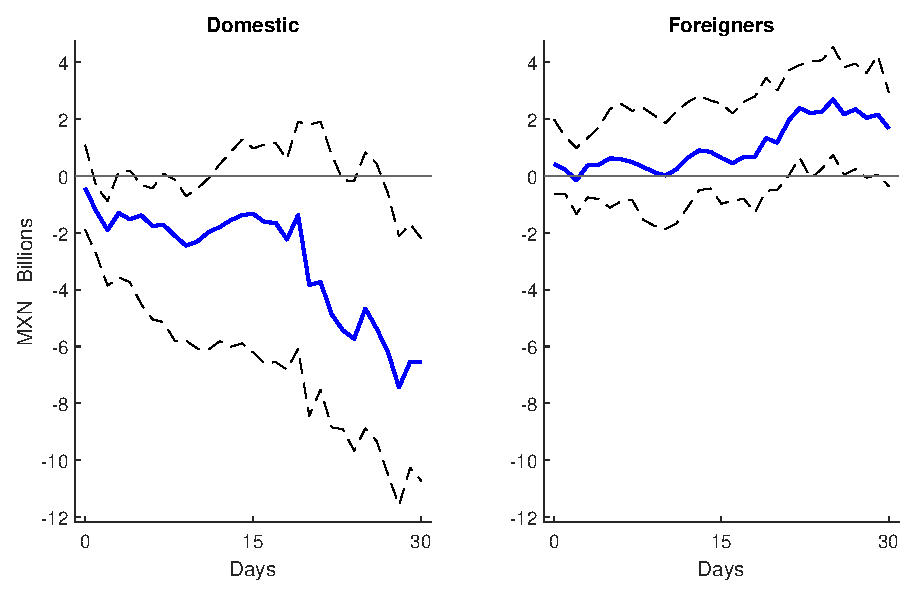
\includegraphics[width=\textwidth]{../Figures/Path11BonosVACateg1post.eps}
						\caption[]{{\small Path Surprise Post}} \label{subfig:Path11BonosVACateg1post}
					\end{subfigure}
				\end{center}
				\fignotes{Coefficient estimates for the response of bonos flows to a 1 basis point target and path tightening surprises from day \(t - 1\) to day \(t + \idxh\), where \(t\) is a day with a monetary policy announcement and \(\idxh = 0, 1, \ldots, 30\). Dashed lines show 95\% bootstrapped confidence bands. The sample starts on January 2011 and ends on \lastobsflwbdm. The top row shows the responses before \breakdatebonos, and the bottom row the responses afterwards.}
			\end{minipage} 
		\end{center}
	\end{figure}
}

The bottom row of figure \ref{fig:LPCetesCateg1sb} shows the cetes flow response after the break date. 
Since 2016Q4, target and path surprises have a rebalancing effect within and across sectors of domestic investors. This can be seen in the widening of the confidence bands for domestic investors (figures \ref{subfig:Target11CetesCateg1post} and \ref{subfig:Path11CetesCateg1post}), and for some specific types (see pension funds in figure \ref{fig:LPCetesCateg2sb}). Moreover, the lower exposure of foreign investors to the cetes market after 2016Q4 is reflected in an essential non-response and thinner confidence bands.

Figure \ref{fig:LPBonosVACateg1sb} shows the persistence of the bonos flow response before and after the break date. 
Before 2021Q1 (top row), domestic investors indistinctly rebalance their bonos portfolios in response to target and path surprises (wide confidence bands). Similarly for foreign investors in response to target surprises, yet they are particularly responsive to path surprises: they buy bonos on the day of the surprise and a few days later. 
After 2021Q1 (bottom row), the response of foreign investors to path surprises remains practically the same, which is reasonable given that their exposure to bonos is still significant and that the break date for bonos is not related to them; the difference is that now domestic investors clearly take the other side of the market (by selling bonos) following a path tightening surprise, mainly driven by the non-financial sector (see figure \ref{subfig:Path11BonosVACateg2post}).\footnote{In figure \ref{subfig:Path11BonosVACateg1post}, one month after the surprise and with wide confidence bands, the magnitude of the average response of domestic investors may end up being larger than that of foreigners. In such a case, a governmental entity, for instance, may be able absorb to the excess supply.}

These results have two important implications. First, foreign investors clearly participate in the transmission of the local monetary policy. 
Taking together the responses of cetes and bonos flows before their respective break dates gives an interesting dynamic: in response to a tightening in the monetary stance, domestic investors position themselves in the short end of the yield curve, while foreign investors prefer to have exposure to the long end.\footnote{Figure \ref{fig:LPUdibonosCateg1} shows that foreigners also sell udibonos after a target tightening surprise.} 
This dynamic may reflect their different investment profiles as the non-financial sector may have a shorter investment horizon than foreign investors, and may explain the large response of the yield curve to path surprises documented in figure \ref{subfig:Path11YCpost}. 

Second, investors take time to rebalance their portfolios to surprises in monetary policy. Cetes and bonos investors rarely react on the day of an announcement. They rebalance their portfolios in the following days, either slowly since the surprise or until after a few days later. Moreover, the effects are not only statistically but also economically significant. In particular, the response to a 1 bp increase in the surprises can represent up to 70\% of a standard deviation of the flows (e.g. compare table \ref{tab:summflowsdy} and figure \ref{subfig:Path11CetesCateg1pre}). Moreover, the sluggish response of the flows supports the evidence of a delayed response in asset prices reported in section \ref{sec:persistencefxyc} and is consistent with the literature on slow-moving capital in asset pricing \parencite{Duffie:2010}.

In summary, target and path surprises trigger a heterogeneous response on different markets and investors. Moreover, the relative influence of each policy can change over time depending on macroeconomic conditions and institutional arrangements. They therefore have an equally important role in the transmission of monetary policy.


\section{Concluding Remarks}\label{sec:conclusions}

This paper uses a new high-frequency dataset to identify monetary policy surprises in an emerging economy. The evidence shows that the central bank conducts monetary policy by adjusting its current policy rate \textit{and} by managing expectations about its future path via statements, both of which strongly and persistently influence asset prices and the portfolio flows of domestic and foreign investors. Moreover, their relative influence can change over time depending on macroeconomic conditions and institutional arrangements. 
The multidimensionality of monetary policy is therefore not exclusive to central banks in advanced economies and does not require the zero lower bound to be binding. 

Having the ability to manage market expectations about the future path of the policy rate via statements can enhance the conduct of monetary policy in emerging markets. For instance, by communicating information about future policy, emerging market central banks can influence medium- and long-term interest rates, which are relevant for the spending decisions of households and businesses.

Given the importance of statements documented here, central banks in emerging markets can follow best practices in monetary policy communications, including brief, clear and concise language without compromising the main message. References to non-monetary policy issues (e.g. structural reforms) should be minimal, if any.\footnote{On this regard, Banxico committed to issue clear and concise statements in February 2020. The guidelines are publicly available at  \url{https://www.banxico.org.mx/publicaciones-y-prensa/miscelaneos/\%7B4C09D772-2CDF-8BD6-3F04-65DE03CA6212\%7D.pdf}.}

The results in this paper can be extended in several directions. 
For instance, decomposing the Mexican sovereign yields can provide additional evidence on the transmission of the two types of monetary policy surprises. In addition, given how foreign investors rebalance their portfolios in response to local monetary policy surprises, policymakers could be interested in the interaction of target and path surprises with different macroprudential policies, including capital controls. Finally, more research is needed to assess the extent to which the results reported here apply to other emerging markets.


\uspunctuation
\begin{singlespace}
	\printbibliography
\end{singlespace}

%---------------------------------------------------------------
% Online Appendix
%---------------------------------------------------------------
\newpage
\begin{appendices}
	
	\setcounter{page}{1}
	\renewcommand{\thetable}{A.\arabic{table}}
	\renewcommand\thefigure{A.\arabic{figure}}
	
	\section*{} \label{sec:apptblsfigs}
	\setcounter{table}{0}
	\setcounter{figure}{0}
	\begin{center}
		{\Large \textbf{Online Appendix}
			
			Do Central Bank Words Matter in Emerging Markets? Evidence from Mexico}
	\end{center}
	
	\begin{normalsize}
		\begin{table}[tbph]
			\begin{center}
				\caption{Summary Statistics for Cetes, Bonos and Udibonos Flows} \label{tab:summflowsdy}
				\begin{threeparttable}
					\begin{tabularx}{0.95\linewidth}{l*{5}C}
						\toprule
						                    &        Mean&   Std. Dev.&        Min.&        Max.&        Obs.\\
						\midrule
						Cetes: Banks        &       0.027&       11.65&      -75.25&       64.35&       3,144\\
						Cetes: Mutual Funds &       0.027&        7.92&      -44.76&       34.34&       3,144\\
						Cetes: Pension Funds&       0.033&        4.75&      -21.20&       48.32&       3,144\\
						Cetes: Insurers     &       0.012&        0.99&       -8.36&        7.99&       3,144\\
						Cetes: Non-Financial&       0.102&       11.83&      -54.98&       60.78&       3,144\\
						Cetes: Domestic     &       0.212&       11.36&     -108.29&      106.92&       3,144\\
						Cetes: Foreigners   &       0.026&        8.24&     -108.45&       37.69&       3,144\\\midrule
						Bonos: Banks        &       0.112&       28.35&     -293.13&      250.35&       3,144\\
						Bonos: Mutual Funds &       0.010&       11.93&      -52.28&       42.09&       3,144\\
						Bonos: Pension Funds&       0.210&        6.88&      -40.57&       30.95&       3,144\\
						Bonos: Insurers     &       0.019&        1.28&      -12.37&       12.32&       3,144\\
						Bonos: Non-Financial&       0.124&       23.24&     -222.01&      247.97&       3,144\\
						Bonos: Domestic     &       0.538&       12.08&     -182.09&       81.31&       3,144\\
						Bonos: Foreigners   &       0.289&        9.40&      -73.02&      112.74&       3,144\\\midrule
						Udibonos: Banks     &       0.000&        0.88&      -10.37&        8.07&       3,144\\
						Udibonos: Mutual Funds&       0.001&        0.75&       -4.69&        4.18&       3,144\\
						Udibonos: Pension Funds&       0.048&        0.52&       -7.09&        3.85&       3,144\\
						Udibonos: Insurers  &       0.019&        0.13&       -1.97&        2.45&       3,144\\
						Udibonos: Non-Financial&       0.012&        1.00&      -11.26&        5.94&       3,144\\
						Udibonos: Domestic  &       0.081&        1.07&      -27.09&        3.35&       3,144\\
						Udibonos: Foreigners&       0.003&        0.17&       -1.84&        1.41&       3,144\\
						\bottomrule
						\addlinespace[.75ex]
					\end{tabularx}
					\tabnote{This table shows summary statistics for different categories of daily flows of cetes, bonos (after adjusting for valuation effects) and udibonos. The flows are obtained as the daily change in the holdings of the respective security. The flows for cetes and bonos are expressed in billions of Mexican pesos, and those for udibonos in billions of UDI (an inflation-linked index). The sample starts on January 2011 and ends on \lastobsflwbdm.}
				\end{threeparttable}
			\end{center}
		\end{table}
	\end{normalsize}
	
	\begin{normalsize}
		\begin{table}
			\begin{center}
				\caption{Structural Break Tests for Portfolio Flows} \label{tab:sbreaksflows} %: Intraday Data
				\begin{threeparttable}
					\begin{tabularx}{0.95\linewidth}{l*{6}C}
						\toprule
						            &\multicolumn{2}{c}{Cetes} &\multicolumn{2}{c}{Bonos} & \multicolumn{2}{c}{Udibonos}\\                                        \cmidrule(lr){2-3}\cmidrule(lr){4-5}\cmidrule(lr){6-7}
						\(h\)       &    Domestic&     Foreign&    Domestic&     Foreign&    Domestic&     Foreign\\
						\cmidrule(lr){1-7}
						0           &           .&           .&           .&           .&           .&           .\\
						1           &           .&           .&           .&           .&           .&           .\\
						2           &           .&           .&           .&           .&           .&           .\\
						3           &    08/12/21\(^{*}\)&           .&           .&           .&           .&           .\\
						4           &           .&           .&    08/12/21\(^{*}\)&           .&           .&           .\\
						5           &           .&           .&           .&           .&           .&           .\\
						6           &           .&           .&           .&           .&           .&           .\\
						7           &           .&           .&           .&           .&           .&           .\\
						8           &           .&           .&           .&           .&           .&           .\\
						9           &           .&           .&           .&           .&           .&           .\\
						10          &           .&           .&           .&           .&           .&           .\\
						11          &           .&           .&           .&           .&           .&           .\\
						12          &           .&           .&           .&           .&           .&           .\\
						13          &           .&           .&           .&           .&           .&           .\\
						14          &           .&           .&           .&           .&           .&           .\\
						15          &           .&           .&           .&           .&           .&           .\\
						16          &           .&    07/11/14\(^{**}\)&           .&           .&           .&           .\\
						17          &           .&    06/04/15\(^{**}\)&           .&           .&           .&    01/18/13\(^{*}\)\\
						18          &           .&    06/04/15\(^{*}\)&           .&           .&           .&           .\\
						19          &           .&    06/06/14\(^{*}\)&           .&           .&           .&           .\\
						20          &           .&    12/15/16\(^{**}\)&           .&           .&           .&           .\\
						21          &           .&    12/15/16\(^{**}\)&           .&           .&           .&           .\\
						22          &           .&    12/15/16\(^{**}\)&           .&           .&           .&           .\\
						23          &           .&    06/06/14\(^{**}\)&           .&           .&           .&           .\\
						24          &           .&    12/15/16\(^{*}\)&           .&           .&           .&           .\\
						25          &           .&           .&           .&           .&           .&           .\\
						26          &           .&           .&           .&           .&           .&           .\\
						27          &           .&           .&    02/11/21\(^{*}\)&           .&           .&           .\\
						28          &           .&    12/15/16\(^{*}\)&    02/11/21\(^{*}\)&           .&           .&           .\\
						29          &           .&           .&           .&           .&           .&           .\\
						30          &           .&           .&    02/11/21\(^{*}\)&           .&           .&           .\\
						\bottomrule
						\addlinespace[.75ex]
					\end{tabularx}
					\tabnote{This table reports the results of the structural break test by \textcite{BaiPerron:2003} to assess whether the effect of monetary policy on portfolio flows has changed over time. The null hypothesis of no structural break in the estimated coefficients \(\beta^{1}_{\idxh}\) and \(\beta^{2}_{\idxh}\) is tested for equation (\ref{eq:nLPflows}) at each horizon \(\idxh = 0, 1, \ldots, 30\). The sample starts on January 2011 and ends on \lastobsflwbdm. The format of the dates is Month/Day/Year. *, **, *** asterisks respectively indicate significance at the 10\%, 5\% and 1\% level.}
				\end{threeparttable}
			\end{center}
		\end{table}
	\end{normalsize}
	
	\begin{figure}
		\caption{Response of the Exchange Rate to Target and Path Surprises} \label{fig:LPFX}
		\centering
		\begin{subfigure}{0.5\textwidth}
			\centering
			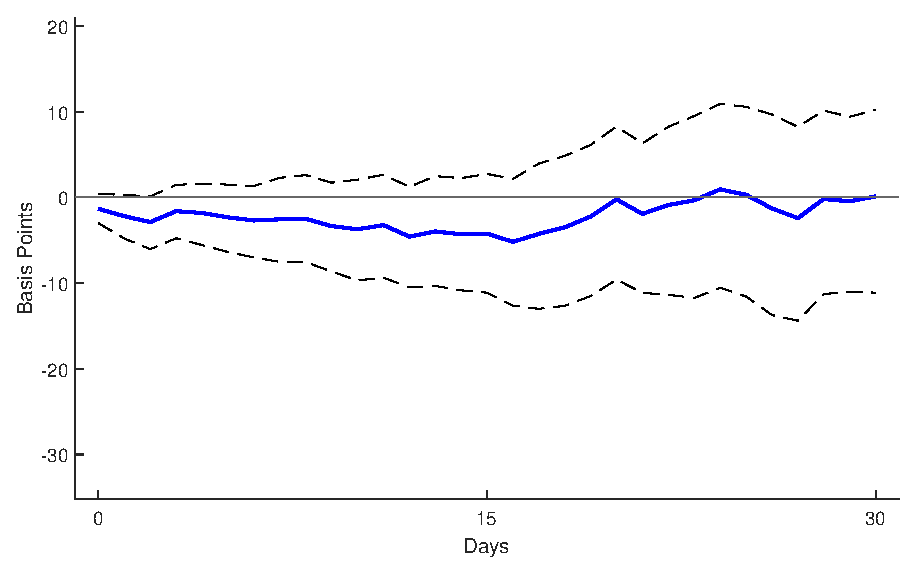
\includegraphics[width=\textwidth]{../Figures/Target11FX.eps} \\
			\caption{Target Surprise} \label{subfig:Target11FX}
		\end{subfigure}%
		\begin{subfigure}{0.5\textwidth}
			\centering
			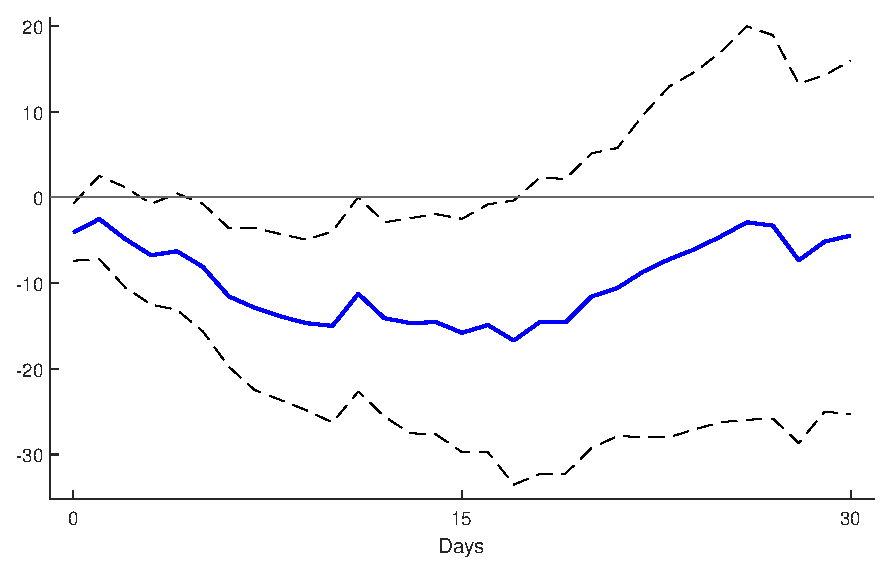
\includegraphics[width=\textwidth]{../Figures/Path11FX.eps} \\
			\caption{Path Surprise} \label{subfig:Path11FX}
		\end{subfigure}
		\fignotes{Coefficient estimates for the response of the exchange rate to a 1 basis point target and path tightening surprises from day \(t - 1\) to day \(t + \idxh\), where \(t\) is a day with a monetary policy announcement and \(\idxh = 0, 1, \ldots, 30\). Dashed lines show 95\% bootstrapped confidence bands. The sample starts on January 2011 and ends on \lastobsflwbdm.}
	\end{figure}
	
	\begin{figure}[tbph]
		\caption{Yield Curve Response to Target and Path Surprises} \label{fig:LPYC}
		\begin{center}
			\begin{minipage}{\linewidth}
				\begin{center}
					\begin{subfigure}[b]{0.475\textwidth}
						\centering
						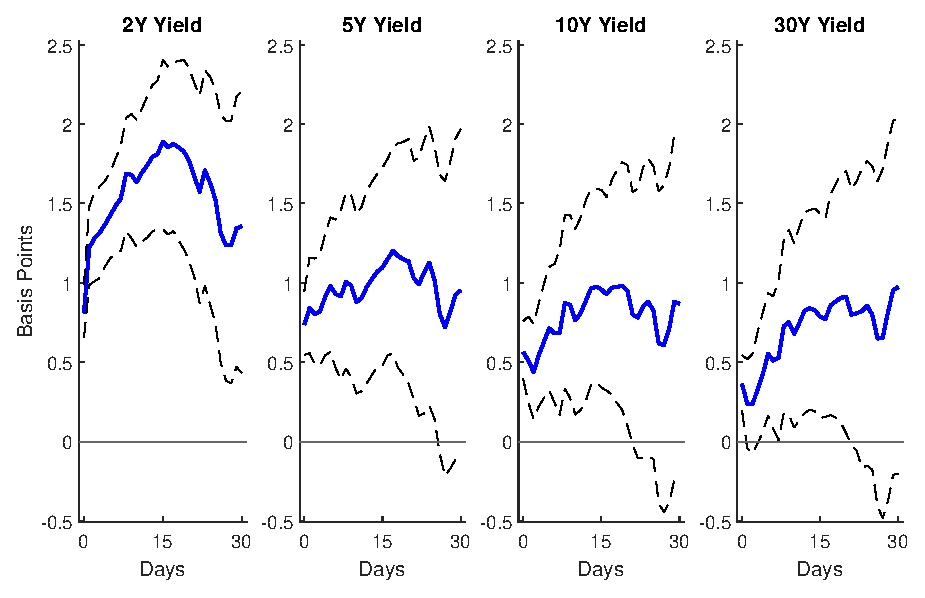
\includegraphics[height=0.35\textheight,width=\textwidth]{../Figures/Target11YC.eps}
						\caption[]{{\small Target Surprise}} \label{subfig:Target11YC}
					\end{subfigure}
					\hfill
					\begin{subfigure}[b]{0.475\textwidth}  
						\centering 
						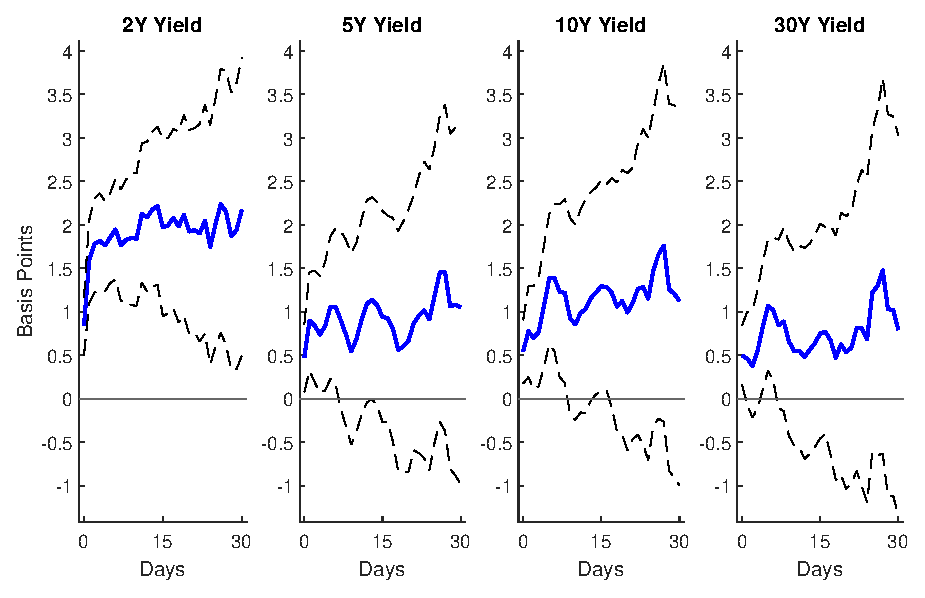
\includegraphics[height=0.35\textheight,width=\textwidth]{../Figures/Path11YC.eps}
						\caption[]{{\small Path Surprise}} \label{subfig:Path11YC}
					\end{subfigure}
				\end{center}
				\fignotes{Coefficient estimates for the response of bond yields to a 1 basis point target and path tightening surprises from day \(t - 1\) to day \(t + \idxh\), where \(t\) is a day with a monetary policy announcement and \(\idxh = 0, 1, \ldots, 30\). Dashed lines show 95\% bootstrapped confidence bands. The sample starts on January 2011 and ends on \lastobsflwbdm.}
			\end{minipage} 
		\end{center}
	\end{figure}
	
	\begin{figure}[!htb]
		\caption{Holdings of Cetes and Bonos by Investor Residence} \label{fig:frgvsdomctsbnd}
		\begin{center}
			\begin{minipage}{0.9\linewidth}
				\begin{center}
					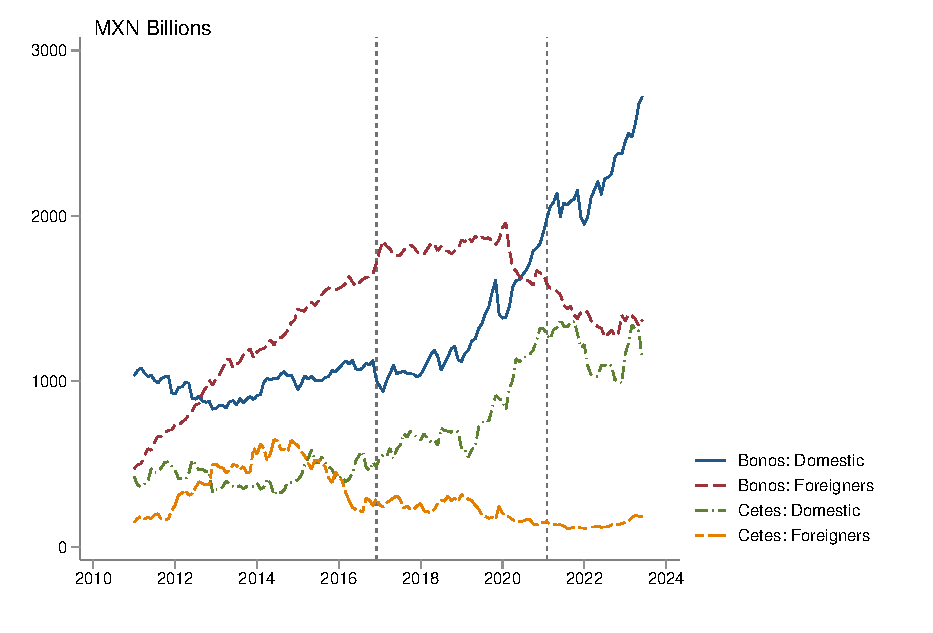
\includegraphics[width=1\textwidth,height=.3\textheight]{../Figures/frgvsdomctsbnd} \\
				\end{center}
				\fignotes{This figure shows the net holdings of Mexican Treasury bills (cetes) and fixed-rate sovereign bonds (bonos) by investor residence from January 2011 to \lastobsflwbdm. Vertical lines indicate break dates, see text for details.}
			\end{minipage}
		\end{center}
	\end{figure}
	
	\begin{figure}[b]
		\caption{Holdings of Cetes by Type of Investor} \label{fig:categscts}
		\begin{center}
			\begin{minipage}{0.9\linewidth}
				\begin{center}
					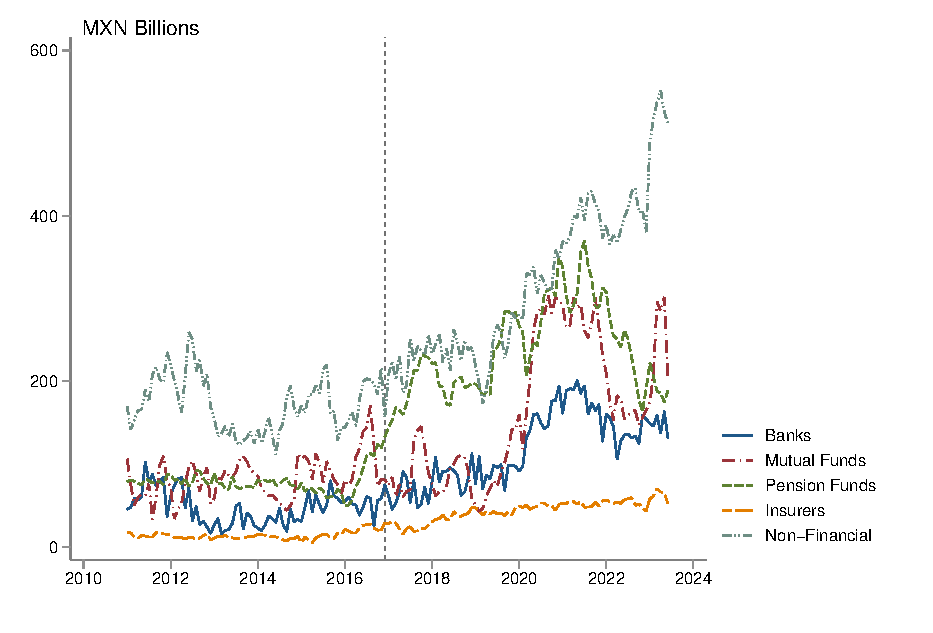
\includegraphics[width=1\textwidth,height=.3\textheight]{../Figures/categscts} \\
				\end{center}
				\fignotes{This figure shows the net holdings of Mexican Treasury bills (cetes) by type of domestic investor from January 2011 to \lastobsflwbdm. The vertical line indicates a break date, see text for details.}
			\end{minipage}
		\end{center}
	\end{figure}
	
	\begin{figure}[!htb]
		\caption{Holdings of Bonos by Type of Investor} \label{fig:categsbnd}
		\begin{center}
			\begin{minipage}{0.9\linewidth}
				\begin{center}
					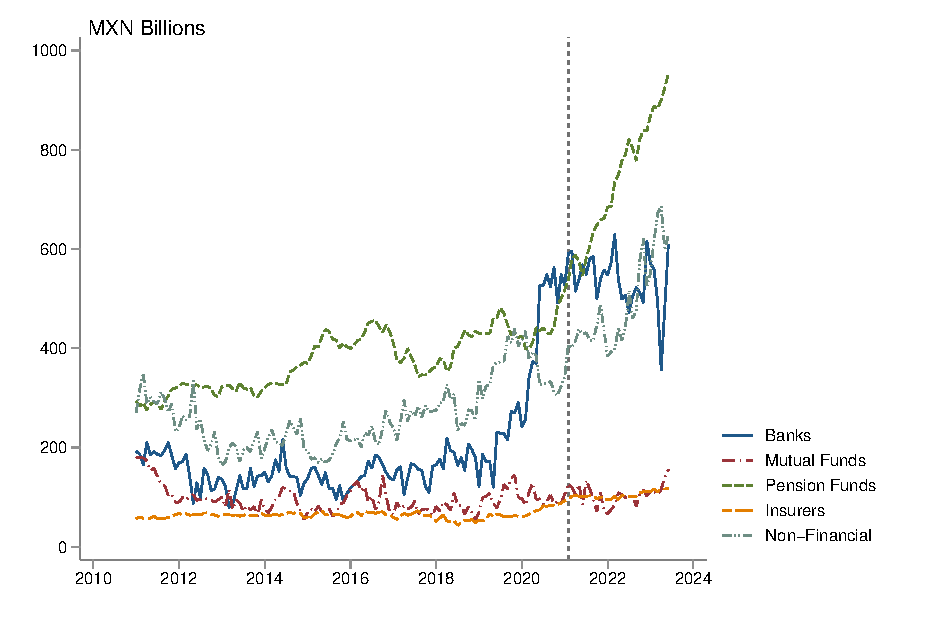
\includegraphics[width=1\textwidth,height=.3\textheight]{../Figures/categsbnd} \\
				\end{center}
				\fignotes{This figure shows the net holdings of fixed-rate Mexican sovereign bonds (bonos) by type of domestic investor from January 2011 to \lastobsflwbdm. The vertical line indicates a break date, see text for details.}
			\end{minipage}
		\end{center}
	\end{figure}
	
	\begin{figure}[!htb]
		\caption{Holdings of Udibonos by Investor Residence} \label{fig:frgvsdomudi}
		\begin{center}
			\begin{minipage}{0.9\linewidth}
				\begin{center}
					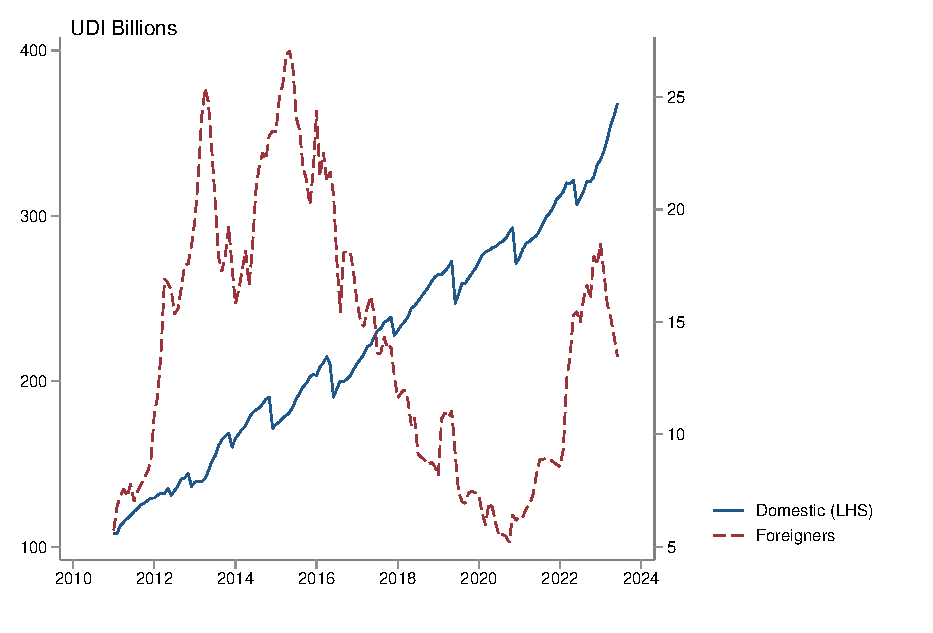
\includegraphics[width=1\textwidth,height=.3\textheight]{../Figures/frgvsdomudi} \\
				\end{center}
				\fignotes{This figure shows the net holdings of Mexican inflation-protected bonds (udibonos) by investor residence from January 2011 to \lastobsflwbdm.}
			\end{minipage}
		\end{center}
	\end{figure}
	
	\begin{figure}[!htb]
		\caption{Holdings of Udibonos by Type of Investor} \label{fig:categsudi}
		\begin{center}
			\begin{minipage}{0.9\linewidth}
				\begin{center}
					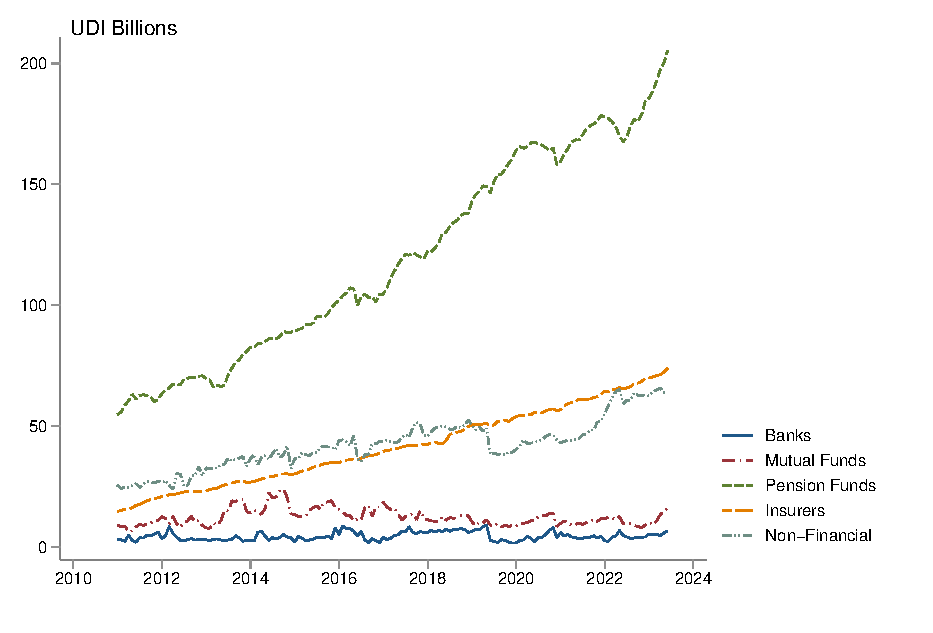
\includegraphics[width=1\textwidth,height=.3\textheight]{../Figures/categsudi} \\
				\end{center}
				\fignotes{This figure shows the net holdings of inflation-protected bonds (udibonos) by type of domestic investor from January 2011 to \lastobsflwbdm.}
			\end{minipage}
		\end{center}
	\end{figure}
	
	\begin{figure}
		\caption{Cetes Flow Response to Target and Path Surprises by Investor Residence} \label{fig:LPCetesCateg1}
		\begin{center}
			\begin{minipage}{\linewidth}
				\begin{center}
					\begin{subfigure}[b]{0.475\textwidth}
						\centering
						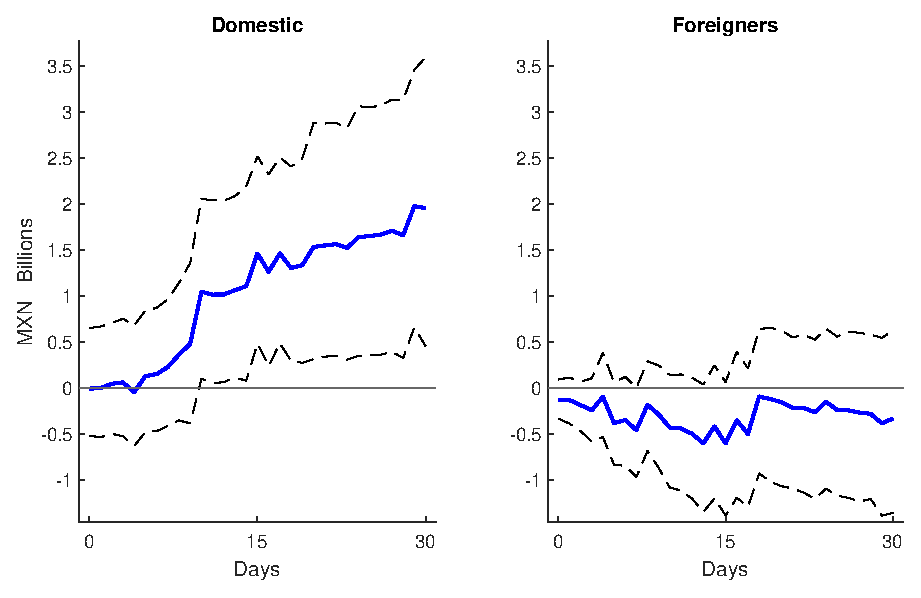
\includegraphics[width=\textwidth]{../Figures/Target11CetesCateg1.eps}
						\caption[]{{\small Target Surprise}} \label{subfig:Target11CetesCateg1}
					\end{subfigure}
					\hfill
					\begin{subfigure}[b]{0.475\textwidth}  
						\centering 
						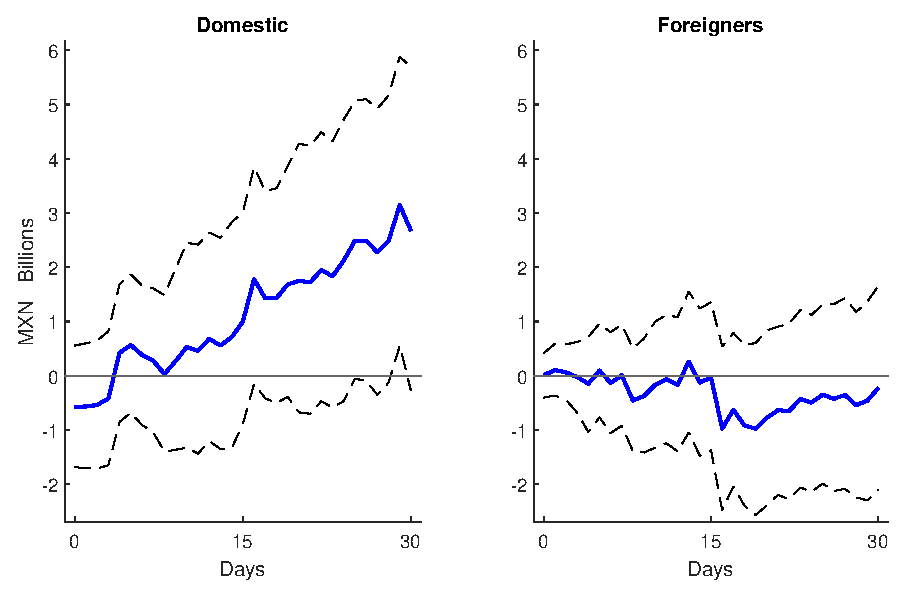
\includegraphics[width=\textwidth]{../Figures/Path11CetesCateg1.eps}
						\caption[]{{\small Path Surprise}} \label{subfig:Path11CetesCateg1}
					\end{subfigure}
				\end{center}
				\fignotes{Coefficient estimates for the response of cetes flows to a 1 basis point target and path tightening surprises from day \(t - 1\) to day \(t + \idxh\), where \(t\) is a day with a monetary policy announcement and \(\idxh = 0, 1, \ldots, 30\). Dashed lines show 95\% bootstrapped confidence bands. The sample starts on January 2011 and ends on \lastobsflwbdm.}
			\end{minipage} 
		\end{center}
	\end{figure}
	
	\begin{figure}
		\caption{Bonos Flow Response to Target and Path Surprises by Investor Residence} \label{fig:LPBonosVACateg1}
		\begin{center}
			\begin{minipage}{\linewidth}
				\begin{center}
					\begin{subfigure}[b]{0.475\textwidth}
						\centering
						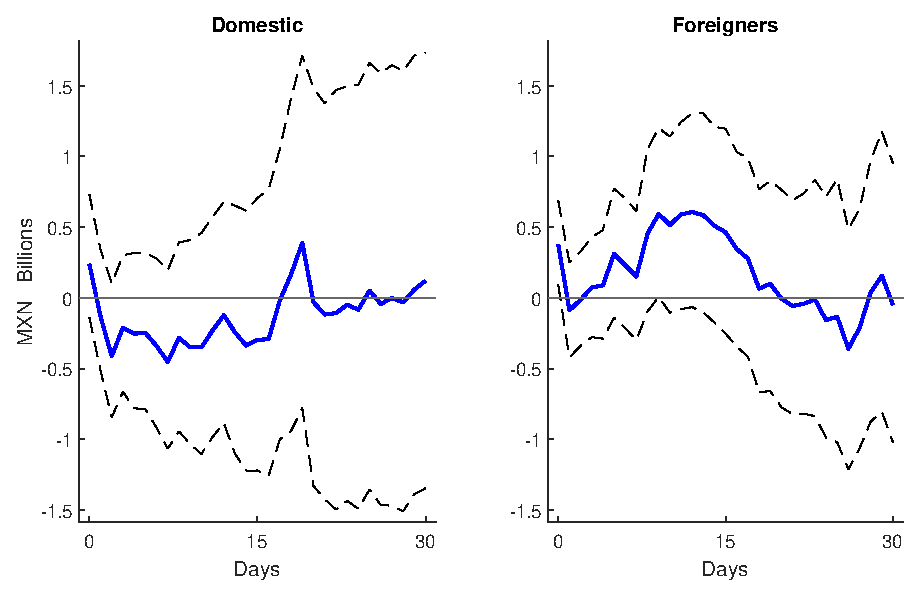
\includegraphics[width=\textwidth]{../Figures/Target11BonosVACateg1.eps}
						\caption[]{{\small Target Surprise}} \label{subfig:Target11BonosVACateg1}
					\end{subfigure}
					\hfill
					\begin{subfigure}[b]{0.475\textwidth}  
						\centering 
						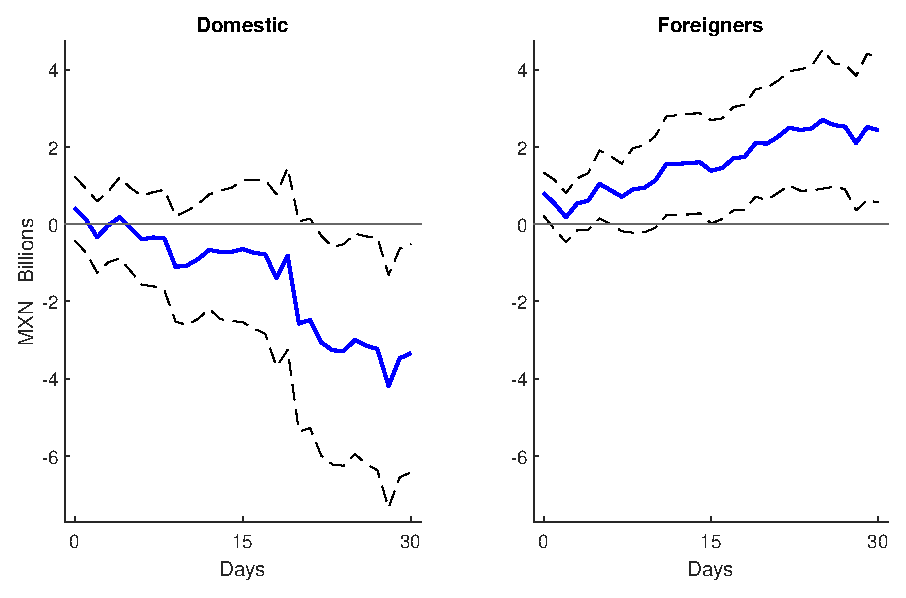
\includegraphics[width=\textwidth]{../Figures/Path11BonosVACateg1.eps}
						\caption[]{{\small Path Surprise}} \label{subfig:Path11BonosVACateg1}
					\end{subfigure}
				\end{center}
				\fignotes{Coefficient estimates for the response of bonos flows to a 1 basis point target and path tightening surprises from day \(t - 1\) to day \(t + \idxh\), where \(t\) is a day with a monetary policy announcement and \(\idxh = 0, 1, \ldots, 30\). Dashed lines show 95\% bootstrapped confidence bands. The sample starts on January 2011 and ends on \lastobsflwbdm.}
			\end{minipage} 
		\end{center}
	\end{figure}
	
	\begin{figure}
		\caption{Udibonos Flow Response to Target and Path Surprises by Investor Residence} \label{fig:LPUdibonosCateg1}
		\begin{center}
			\begin{minipage}{\linewidth}
				\begin{center}
					\begin{subfigure}[b]{0.475\textwidth}
						\centering
						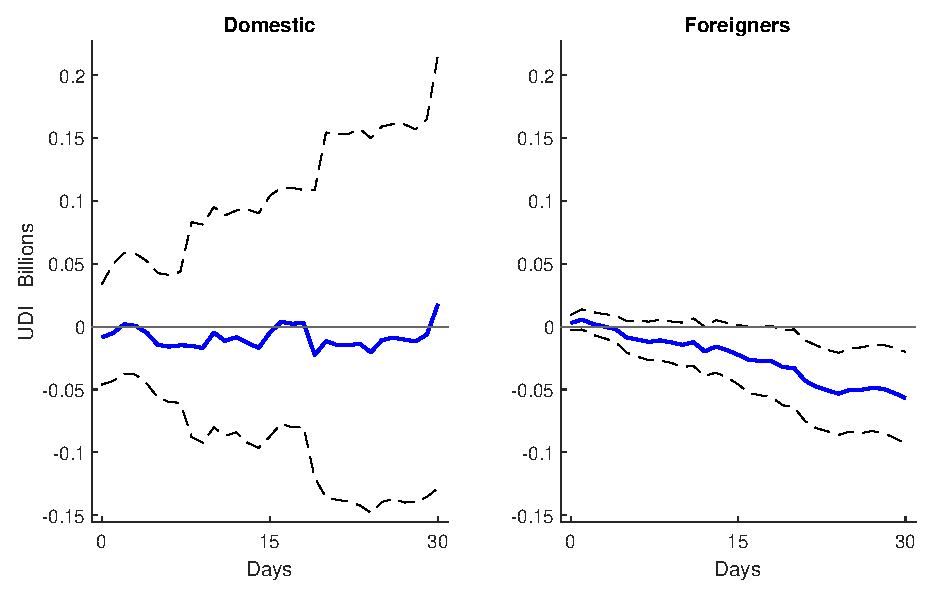
\includegraphics[width=\textwidth]{../Figures/Target11UdibonosCateg1.eps}
						\caption[]{{\small Target Surprise}} \label{subfig:Target11UdibonosCateg1}
					\end{subfigure}
					\hfill
					\begin{subfigure}[b]{0.475\textwidth}  
						\centering 
						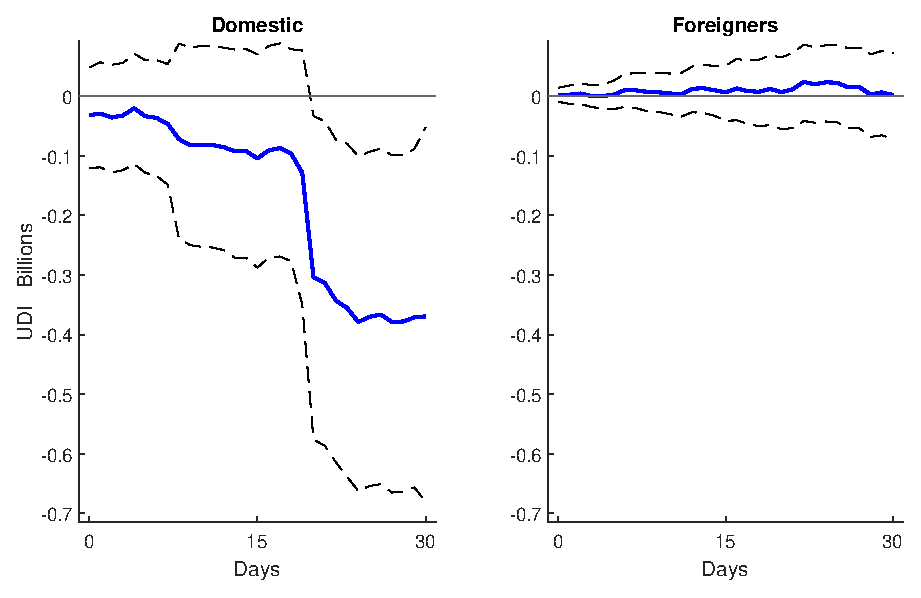
\includegraphics[width=\textwidth]{../Figures/Path11UdibonosCateg1.eps}
						\caption[]{{\small Path Surprise}} \label{subfig:Path11UdibonosCateg1}
					\end{subfigure}
				\end{center}
				\fignotes{Coefficient estimates for the response of udibonos flows to a 1 basis point target and path tightening surprises from day \(t - 1\) to day \(t + \idxh\), where \(t\) is a day with a monetary policy announcement and \(\idxh = 0, 1, \ldots, 30\). Dashed lines show 95\% bootstrapped confidence bands. The sample starts on January 2011 and ends on \lastobsflwbdm.}
			\end{minipage} 
		\end{center}
	\end{figure}
	
	\begin{landscape}
		\begin{figure}[tbph]
			\caption{Cetes Flow Response to Target and Path Surprises by Type of Domestic Investor} \label{fig:LPCetesCateg2sb}
			\begin{center}
				\begin{minipage}{\linewidth}
					\begin{center}
						\begin{subfigure}[b]{0.475\textwidth}
							\centering
							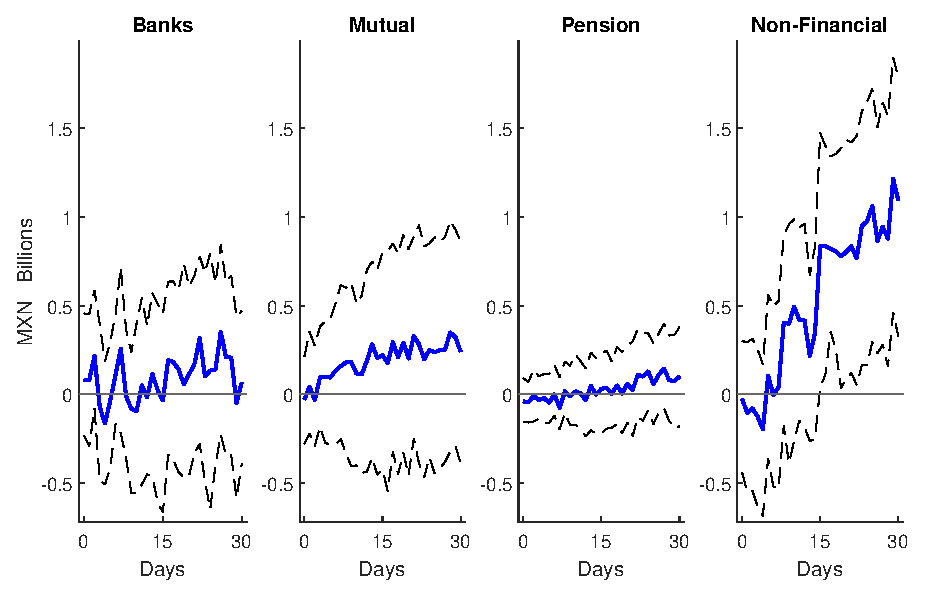
\includegraphics[height=0.35\textheight,width=\textwidth]{../Figures/Target11CetesCateg2pre.eps}
							\caption[]{{\small Target Surprise Pre}} \label{subfig:Target11CetesCateg2pre}
						\end{subfigure}
						\hfill
						\begin{subfigure}[b]{0.475\textwidth}  
							\centering 
							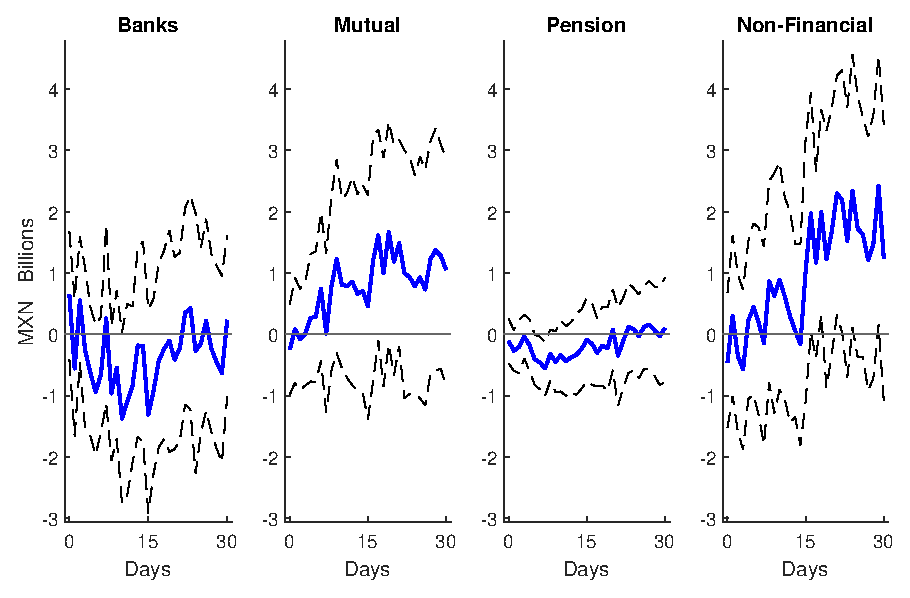
\includegraphics[height=0.35\textheight,width=\textwidth]{../Figures/Path11CetesCateg2pre.eps}
							\caption[]{{\small Path Surprise Pre}} \label{subfig:Path11CetesCateg2pre}
						\end{subfigure}
						\vskip\baselineskip
						\begin{subfigure}[b]{0.475\textwidth}   
							\centering 
							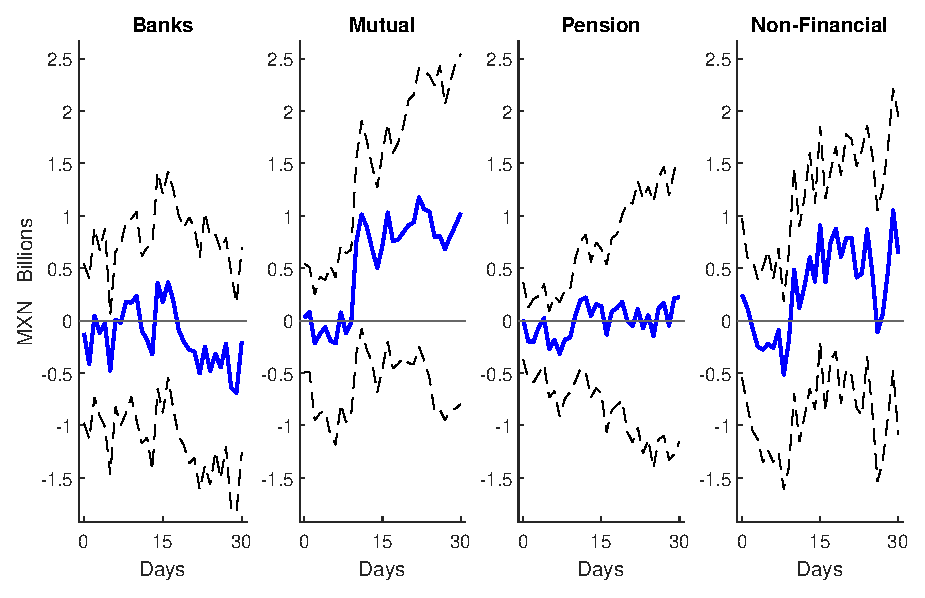
\includegraphics[height=0.35\textheight,width=\textwidth]{../Figures/Target11CetesCateg2post.eps}
							\caption[]{{\small Target Surprise Post}} \label{subfig:Target11CetesCateg2post}
						\end{subfigure}
						\hfill
						\begin{subfigure}[b]{0.475\textwidth}   
							\centering 
							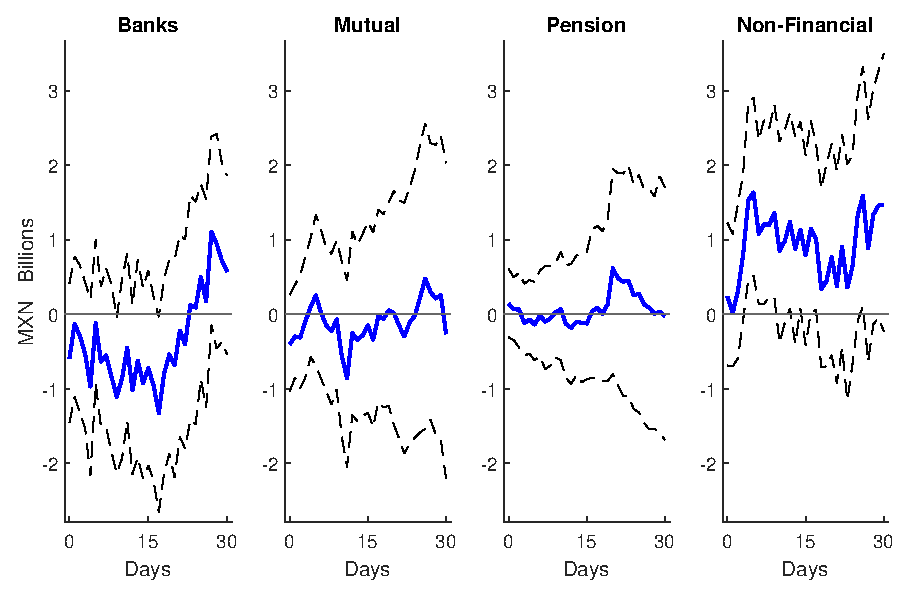
\includegraphics[height=0.35\textheight,width=\textwidth]{../Figures/Path11CetesCateg2post.eps}
							\caption[]{{\small Path Surprise Post}} \label{subfig:Path11CetesCateg2post}
						\end{subfigure}
					\end{center}
					\fignotes{Coefficient estimates for the response of cetes flows to a 1 basis point target and path tightening surprises from day \(t - 1\) to day \(t + \idxh\), where \(t\) is a day with a monetary policy announcement and \(\idxh = 0, 1, \ldots, 30\). Dashed lines show 95\% bootstrapped confidence bands. The sample starts on January 2011 and ends on \lastobsflwbdm. The top row shows the responses before \breakdatecetes, and the bottom row the responses afterwards.}
				\end{minipage} 
			\end{center}
		\end{figure}
	\end{landscape}
	
	\begin{landscape}
		\begin{figure}[tbph]
			\caption{Bonos Flow Response to Target and Path Surprises by Type of Domestic Investor} \label{fig:LPBonosVACateg2sb}
			\begin{center}
				\begin{minipage}{\linewidth}
					\begin{center}
						\begin{subfigure}[b]{0.475\textwidth}
							\centering
							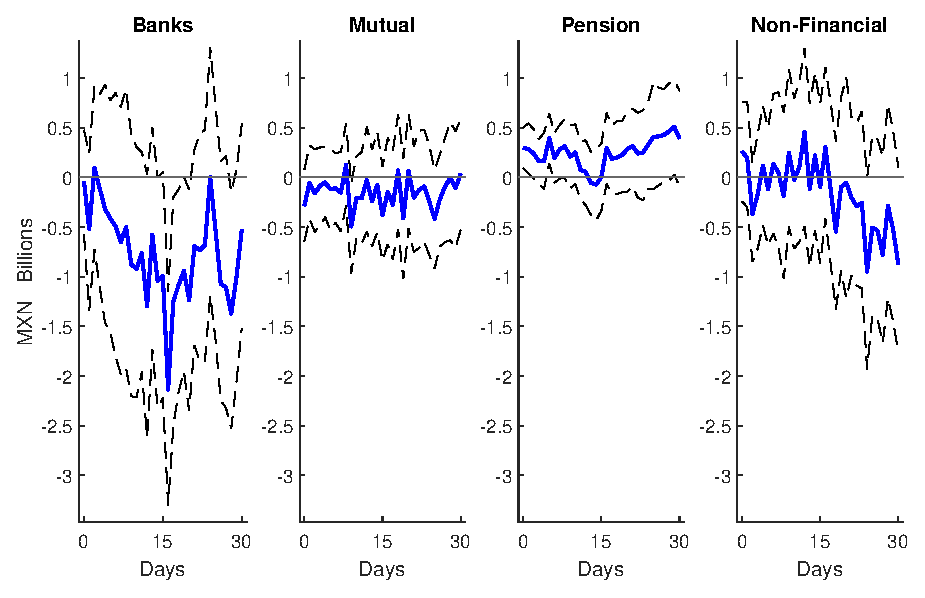
\includegraphics[height=0.35\textheight,width=\textwidth]{../Figures/Target11BonosVACateg2pre.eps}
							\caption[]{{\small Target Surprise Pre}} \label{subfig:Target11BonosVACateg2pre}
						\end{subfigure}
						\hfill
						\begin{subfigure}[b]{0.475\textwidth}  
							\centering 
							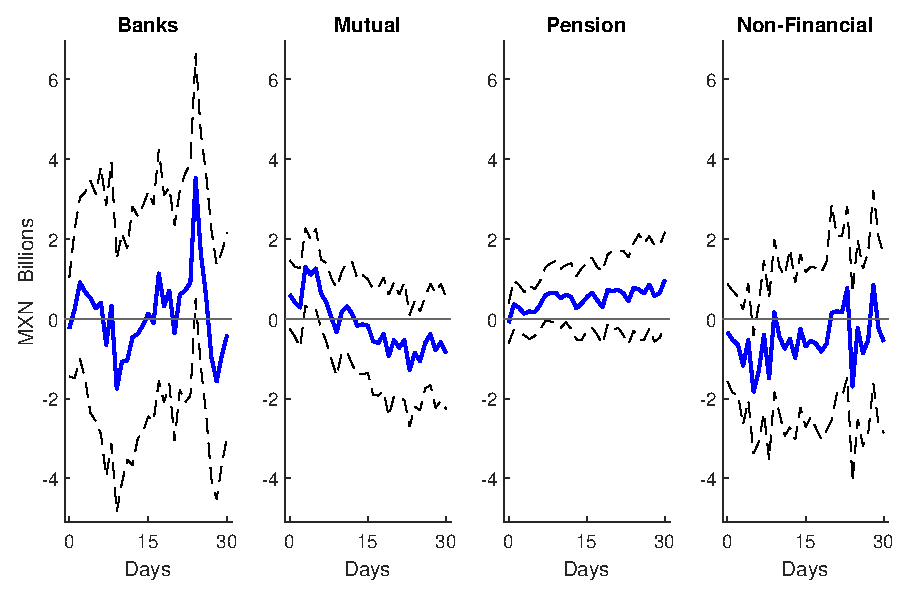
\includegraphics[height=0.35\textheight,width=\textwidth]{../Figures/Path11BonosVACateg2pre.eps}
							\caption[]{{\small Path Surprise Pre}} \label{subfig:Path11BonosVACateg2pre}
						\end{subfigure}
						\vskip\baselineskip
						\begin{subfigure}[b]{0.475\textwidth}   
							\centering 
							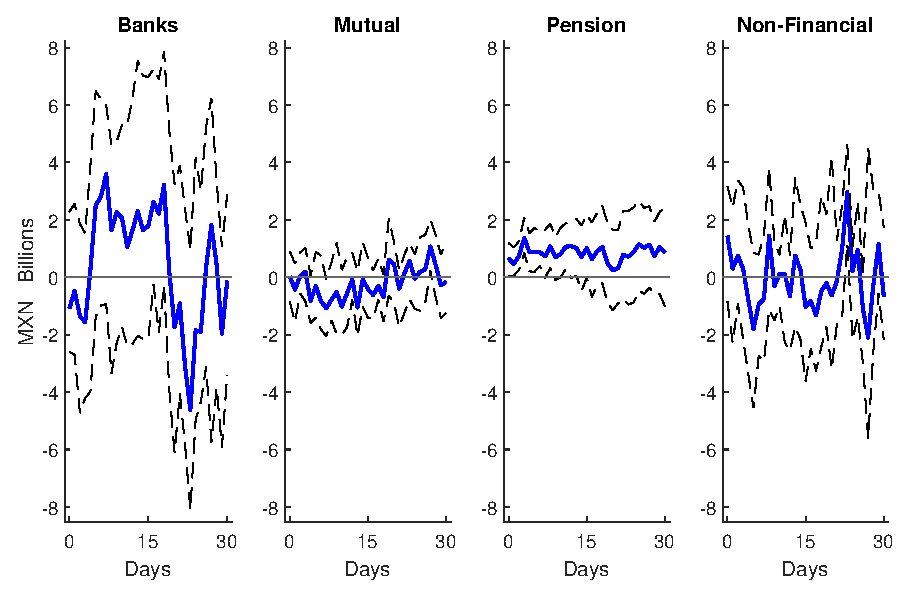
\includegraphics[height=0.35\textheight,width=\textwidth]{../Figures/Target11BonosVACateg2post.eps}
							\caption[]{{\small Target Surprise Post}} \label{subfig:Target11BonosVACateg2post}
						\end{subfigure}
						\hfill
						\begin{subfigure}[b]{0.475\textwidth}   
							\centering 
							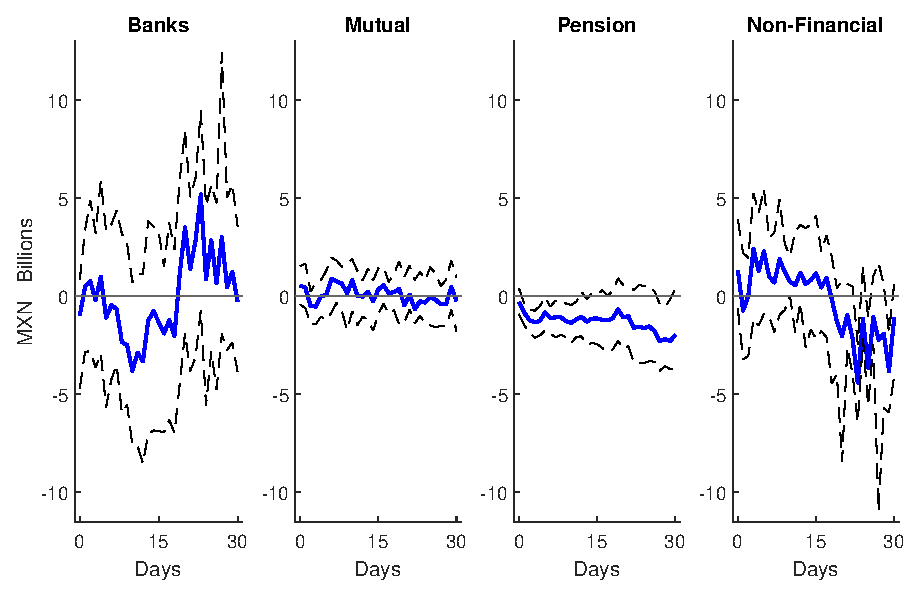
\includegraphics[height=0.35\textheight,width=\textwidth]{../Figures/Path11BonosVACateg2post.eps}
							\caption[]{{\small Path Surprise Post}} \label{subfig:Path11BonosVACateg2post}
						\end{subfigure}
					\end{center}
					\fignotes{Coefficient estimates for the response of bonos flows to a 1 basis point target and path tightening surprises from day \(t - 1\) to day \(t + \idxh\), where \(t\) is a day with a monetary policy announcement and \(\idxh = 0, 1, \ldots, 30\). Dashed lines show 95\% bootstrapped confidence bands. The sample starts on January 2011 and ends on \lastobsflwbdm. The top row shows the responses before \breakdatebonos, and the bottom row the responses afterwards.}
				\end{minipage} 
			\end{center}
		\end{figure}
	\end{landscape}
	
	\begin{landscape}
		\begin{figure}[tbph]
			\caption{Response of Udibonos Flows to Target and Path Surprises by Domestic Institutions} \label{fig:LPUdibonosCateg2}
			\begin{center}
				\begin{minipage}{\linewidth}
					\begin{center}
						\begin{subfigure}[t]{\linewidth}
							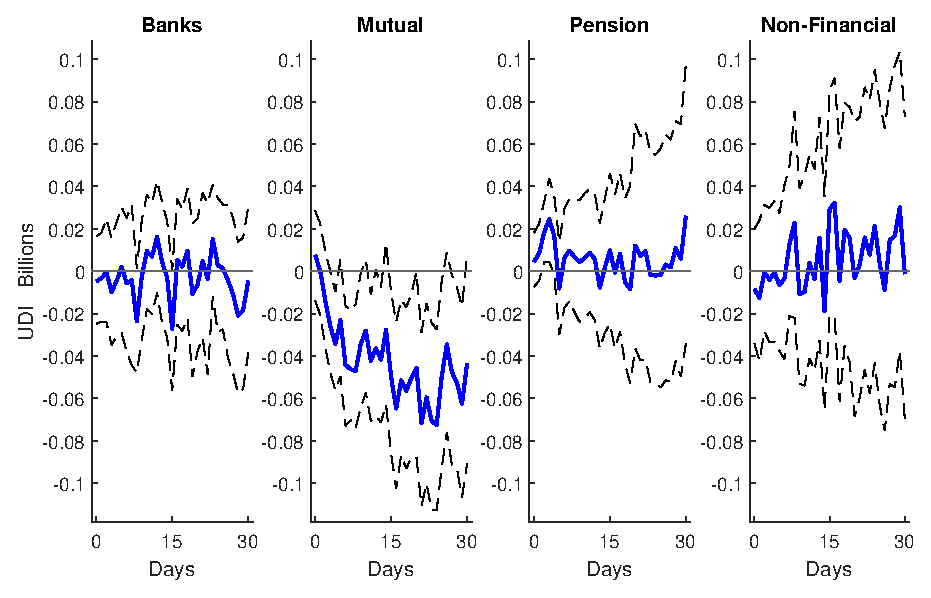
\includegraphics[height=0.33\textheight,width=\linewidth]{../Figures/Target11UdibonosCateg2.eps} \\
							\vspace{-0.35cm}
							\caption{Target  Surprise} \label{subfig:Target11UdibonosCateg2}
							\vspace{0.4cm}
						\end{subfigure}
						
						\vspace{0.1cm}
						
						\begin{subfigure}[t]{\linewidth}
							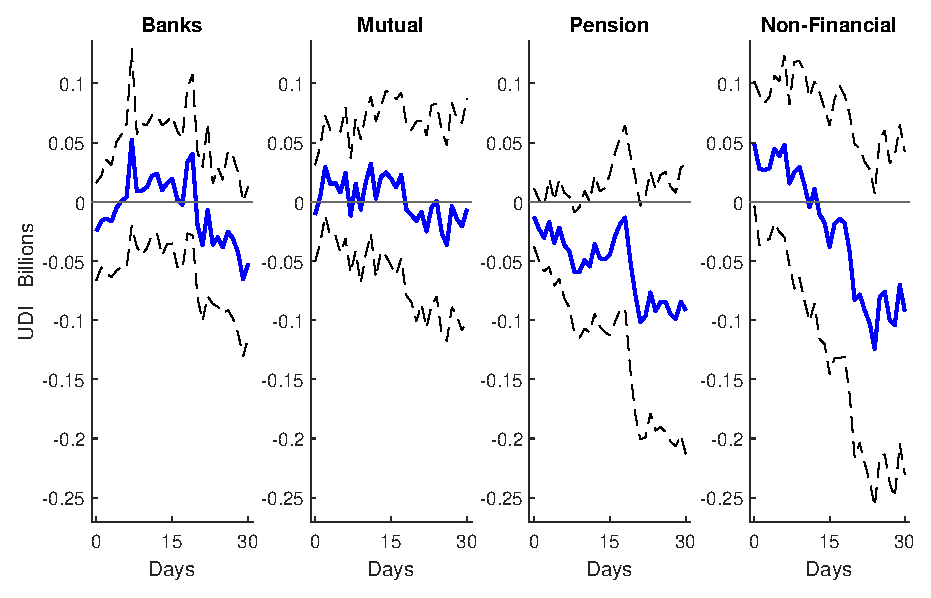
\includegraphics[height=0.33\textheight,width=\linewidth]{../Figures/Path11UdibonosCateg2.eps} \\
							\vspace{-0.35cm}
							\caption{Path Surprise} \label{subfig:Path11UdibonosCateg2}
						\end{subfigure}
						\vspace{-0.45cm}
					\end{center}
					\fignotes{Coefficient estimates for the response of udibonos flows to a 1 basis point target and path tightening surprises from day \(t - 1\) to day \(t + \idxh\), where \(t\) is a day with a monetary policy announcement and \(\idxh = 0, 1, \ldots, 30\). Dashed lines show 95\% bootstrapped confidence bands. The sample starts on January 2011 and ends on \lastobsflwbdm.}
				\end{minipage}
			\end{center}
		\end{figure}
	\end{landscape}

\end{appendices}

\end{document}